%
% Software.tex
%
% LulzBot Mini User Manual
%
% Copyright (C) 2014 Aleph Objects, Inc.
%
% This document is licensed under the Creative Commons Attribution 4.0
% International Public License (CC BY-SA 4.0) by Aleph Objects, Inc.
%

\section{Software Overview}
\index{software}

Aleph Objects, Inc., the maker of the LulzBot\textsuperscript{\miniscule{\texttrademark}} Mini, completely supports free/libre hardware and software. Along with the Mini being a free/libre hardware design, it has been tested to work with 100\% free/libre software. Our source code and design files are hosted on our development server found at \texttt{http://devel.lulzbot.com}.
\glossary{free/libre}{Free/Libre hardware and software can be thought of as "free as in free speech, not just free as in free beer", although most free/libre software is available for no cost. Libre hardware designs can be copied, modified and are usually available for download. Free/Libre software can be used in a similar fashion.}
To operate your desktop 3D printer you will need to install a few software packages onto your PC. You will need a 3D printer host, an \texttt{.STL} to \texttt{.gcode} generator, and optional CAD or 3D modeling software.
\glossary{.gcode}{The file extension for G-Code files}
\glossary{GCODE}{The common name for the most widely used CNC programming language.}
\glossary{CAD}{Computer Aided Design}

\section{Software Types}
\index{Printer Host}
\index{Slicing}
\index{Slicers}
\index{gcode}
\index{g-code}

\begin{description}
\item{Printer Hosts} \hfill \\
Printer Host software is used to control the 3D printer. The program not only allows you to manually move the printer along all the axes, but set temperatures manually, send commands and receive feedback/error messages from the onboard electronics. We recommend that new users start with Cura as it includes a slicing engine as well.

Common Printer Hosts:
\begin{itemize}
\item Cura
\item Printrun (Pronterface)
\item MatterControl
\item OctoPrint
\item Botqueue
\end{itemize}

\item{Slicers} \hfill \\
These programs take the 3-Dimensional model (typically STL/OBJ/etc) and determine the 3D printer toolpath based on the options selected. The slicing engine uses the nozzle diameter, printing and movement speeds, layer height and other variables to determine the coordinates where it needs to move and the rates at which it will do so. This information is exported out of the program as a gcode file. The gcode file is a plain-text file with a series of text-based codes and a list of the complete X,Y and Z axis coordinates used for printing the 3D model. We recommend that new users start with Cura as it includes the printer host as well.

Recommended Slicers:
\begin{itemize}
\item Cura
\item Slic3r
%\item Skeinforge
%\item Sfact
\end{itemize}

\end{description}

\index{GNU/Linux}
\index{Apple OS X}
\index{Windows}
\index{operating system}
All of the following free/libre software packages are available for GNU/Linux, Windows, and Apple OS X. However, we highly recommend using these programs on GNU/Linux.

\index{download}
The required software can be found in the Support/Downloads section at \texttt{LulzBot.com/support/downloads}. You will also find instructions there for installing each program onto your PC. You can also find downloads specific to the LulzBot\textsuperscript{\miniscule{\texttrademark}} Mini 3D printer on the LulzBot\textsuperscript{\miniscule{\texttrademark}} Mini product page.

\index{driver}
\section{Installing Drivers}
Linux and Mac OSX users will not need to install a driver to communicate with the Mini 3D printer. Windows users will need to install the drivers. Using Cura as your printer host and slicing software is recommended, as the drivers will automatically be installed. The drivers can also be downloaded from \texttt{LulzBot.com/support/downloads}. A visual guide showing the driver installation process can be found in our download section as well.

%%%% Change the following section when Cura.tex can be replaced by the standalone version. %%%%

%Testing cleaner section insertion
%\index{Cura}
%%
% Cura.tex
%
% LulzBot Mini User Manual
%
% Copyright (C) 2016 Aleph Objects, Inc.
%
% This document is licensed under the Creative Commons Attribution 4.0
% International Public License (CC BY-SA 4.0) by Aleph Objects, Inc.
%

\section{\texttt{Cura LulzBot Edition}}
\index{Cura}
\index{Cura LulzBot Edition}
\label{Cura}
\glossary{\texttt{Cura}}{Cura LulzBot Edition is a cross-platform software package that combines a slicing engine with a printer host interface.}
\glossary{Slic3r}{Slic3r is a cross-platform 3D model slicing engine. It's used to process the 3 dimensional model into the GCODE (tool path) needed to physically generate the print.}
\glossary{FFF}{Fused Filament Fabrication-- the process of laying down successive layers of extruded filament to create a 3 dimensional object. As each layer of molten plastic is extruded into place, it fuses with the previous layer.}

\subsection{\texttt{Installation and Setup}}
\index{installation}
Cura LulzBot Edition is available for download on our website at \texttt{http://LulzBot.com/cura}. When installing, it is recommended to uninstall any previous versions of Cura you may have been using. Cura is designed for Fused Filament Fabrication (FFF) 3D printers. Fused Filament Fabrication is the term for the process of laying down successive layers of extruded filament to create a 3 dimensional object. As each layer of molten plastic is extruded into place, it fuses with the previous layer.
When first opening Cura, you will be prompted to go through the \texttt{First run wizard}. This will consist of selecting your printer, hot end type, tool head type, and finally your nozzle diameter.

\textcolor{red}{It is important to select the correct printer, hot end, tool head, and nozzle diameter as Cura uses custom profiles and machine settings based upon which printer, hot end, tool head, and nozzle you have.}

\begin{itemize}
\item Download the appropriate installer for your computer operating system. Instructions on installation for each operating system are available at \texttt{http://LulzBot.com/cura}.
\item Install Cura by double clicking on the installer.
%\item Click through the install wizard until it completes.
\item Start Cura by launching it from your list of installed applications. If this is the first time that Cura has been used the ``Configuration Wizard'' window will open.
%\item Once your language has been selected, select \texttt{Next}.
\item Select \texttt{LulzBot Mini}.
%\item Select \texttt{LulzBot\textsuperscript{\miniscule{\textregistered}} TAZ 4 or 5}, then select \texttt{Next}.
%\item Select \texttt{LulzBot TAZ 6}. Press \texttt{Next}.
\item Select \texttt{Standard LulzBot Mini} Press \texttt{Next}.
%\item Select \texttt{Single Extruder v2.1}. Press \texttt{Next}
%\item The final step will be a firmware update. \textcolor{red}{Skip this step if you are not switching to different tool heads.} If you are adding on a different tool head, please be sure to update the firmware.
\item Select finish.
\end{itemize}


\section{\texttt{Quick Print Settings}}
\index{Quick Print Settings}
\begin{figure}[H]
\centering
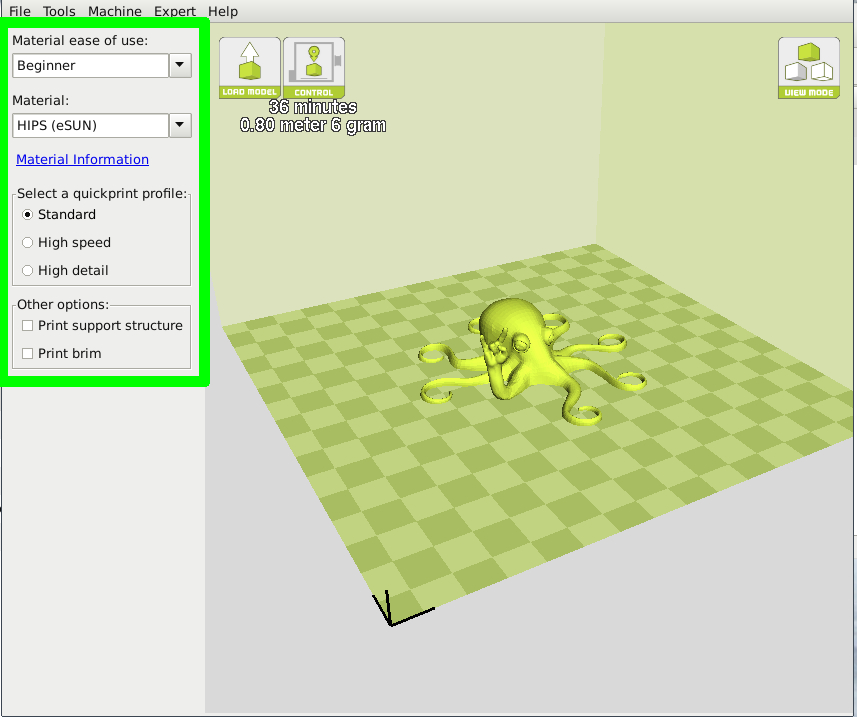
\includegraphics[keepaspectratio=true,angle=0,height=0.4\textheight,width=1.0\textwidth]{QPscreen.jpg}
\caption{Quick Print Settings}
\label{fig:Cura}
\end{figure} 
% (photo highlighting profile, material, diameter, and other)
After setting up Cura for the first time, you will be shown the main interface screen. (Fig. \ref{fig:Cura}, page \pageref{fig:Cura}): 

\subsection{\texttt{Material Selection}}
\index{material selection}
\index{filament}
\index{filament vendors}
We have the different filament types separated by \texttt{Material ease of use.} From the \texttt{Material ease of use} drop down, select \texttt{"All"} to view all our pre-loaded filament slicing profiles. The Mini ships with a filament sample for the first print. Refer to the included Quick Start Guide for the proper ``First Run'' settings.

\subsubsection{\texttt{Different Filament Manufacturers}}
Different manufacturers have different formulations for their specific brand. These different formulations may have different ideal settings. We usually use 6kg - 10kg of filament when developing these profile settings. \textcolor{red}{We highly recommend using the filament brands listed in Cura LulzBot Edition. Beautiful 3D printed objects start with reliable and consistent filament.} Our profiles will be good starting points for other manufacturers but they may not be ideal.

\subsection{\texttt{Selecting a Quick Print Profile}}
\index{quick print profile}
\index{resolution}
\index{layer height}
\glossary{Resolution}{In general terms, the resolution you print at can be determined by the layer height you use. The LulzBot Mini can print at a layer heights of 0.05mm to 0.50mm with the standard tool head.}
The print quality settings can be found in the top left-hand corner of the window. For most filaments, there will be \texttt{Standard}, \texttt{High Speed}, and \texttt{High Detail} options. Some of the more exotic filaments may have fewer profiles.

\begin{description}
\item[\texttt{High detail}] \hfill \\
Designed to give greater detail and finer objects. This will have a smaller layer height, which will make each layer thinner, so that curves seem more natural and walls seem less noticeable. This setting will also require more layers to be laid down, increasing overall print time.
\index{High detail}

\item[\texttt{Standard}] \hfill \\
Designed to give a medium resolution, by increasing the layer height and print speeds. This will make the organic curves slightly more step-like than the fine setting, but will reduce printing time.
\index{Standard}

\item[\texttt{High speed}] \hfill \\
Designed for the fast prints, where overall model finish is not of concern. Most commonly used for quick iteration of designs found in rapid prototyping.
\index{High speed}
\end{description}


%If you are not using Lulzbot supplied filament, update your filament diameter to your specific average filament diameter. Do this by taking 10 to 12 filament diameter measurements from different parts of the reel and averaging them. Update your filament diameter. %You may also want to adjust the temperature, as different manufacturers have different recommended temperatures. % This would be better served in the Full Settings explination.

\subsection{\texttt{Printing Support Material}}
\index{Support Material}
%%%% Saved for standalone Cura Manual %%%%
%The TAZ and Mini are able to print models that have angles and overhangs, even without support material depending on the overhang distance and angle. Turn this option on if your model could benefit from support material.
The LulzBot Mini 3D printer is able to print models that have angles and overhangs, even without support material. This will depend on the overhang distance and angle of your particular model file. Turn this option on if sections of your model are being are extending in mid air. This will build up material underneath the portion extending in mid air, preventing gravity from making the object droop.

\subsection{\texttt{Brim}}
\index{Brim}
Brim is used to increase surface area of the part you're printing, thereby ensuring proper part adhesion. This will print a single layer high edge around the base of the part, helping first layer adhesion and minimizing warping.

\subsection{\texttt{Load Model File}}
\index{Load Model}
\index{load model}
\index{3D models}
\index{STL}
\index{OBL}
\index{AMF}
Select the model you would like to print. Either use the \texttt{Load Model} button or select \texttt{File} > \texttt{Load Model}. Once the file has been loaded, you will see a 3D rendering of your object on the build platform. Select the model to see the various options. 

\subsection{\texttt{Model Orientation}}
\index{Orientation}
Move your model to change where it is printed on the build plate. Do this by left clicking on the model and dragging it to the desired location. The \texttt{black outlined corner represents the lower left hand corner of the build plate on your printer.} You can view your model from different angles by holding down the right mouse button and dragging %Not sure if this last sentence should be reworked or put in a separate section.
\begin{figure}[H]
\centering
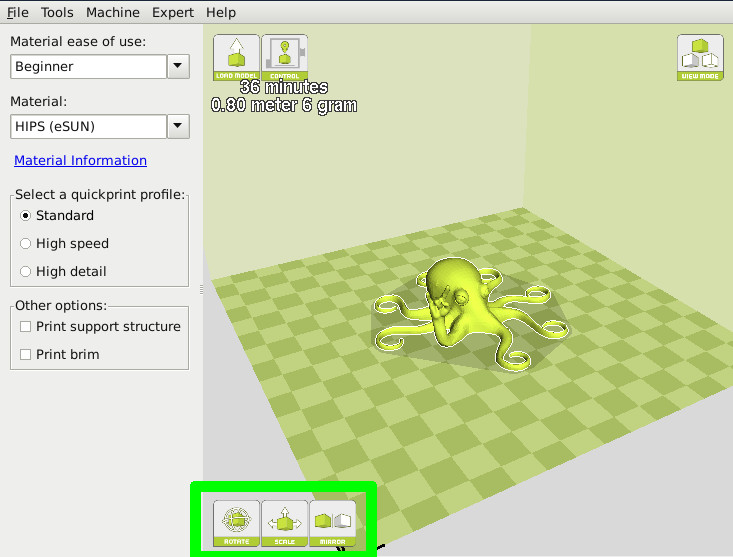
\includegraphics[keepaspectratio=true,angle=0,height=0.4\textheight,width=1.0\textwidth]{optionsRSM1.jpg}
\caption{Options after selecting model}
\label{fig:Orientation}
\end{figure}

\subsubsection{\texttt{Rotate}}
%%%% Alternate explanation %%%%
%The \texttt{Rotate} button will give you the ability orient your model in along all three axes. Once you click the rotate button, three circles will surround your model. The red circle will allow you to rotate in the XY plane. The Yellow circle will rotate in the XZ plane. The Green circle will rotate in the YZ plane.
\definecolor{yellow1}{cmyk}{0,0,1,0.30}
\definecolor{green1}{rgb}{0.30,1,0.30}
The \texttt{Rotate} button will give you the ability to orient your model in along all three axes. Once you click the rotate button, three circles will surround your model. The \textcolor{red}{red circle} will allow you to rotate around the \textcolor{red}{Z-axis}. The \textcolor{yellow1}{Yellow circle} will rotate around the \textcolor{yellow1}{Y-axis}. The \textcolor{green}{Green circle} will rotate around the \textcolor{green}{X-axis}. Cura defaults to 15 degree increments. Hold \texttt{Shift} to rotate by \texttt{One Degree Increments}. (Fig. \ref{fig:Rotating your Model}, page \pageref{fig:Rotating your Model})

\begin{figure}[H]
\centering
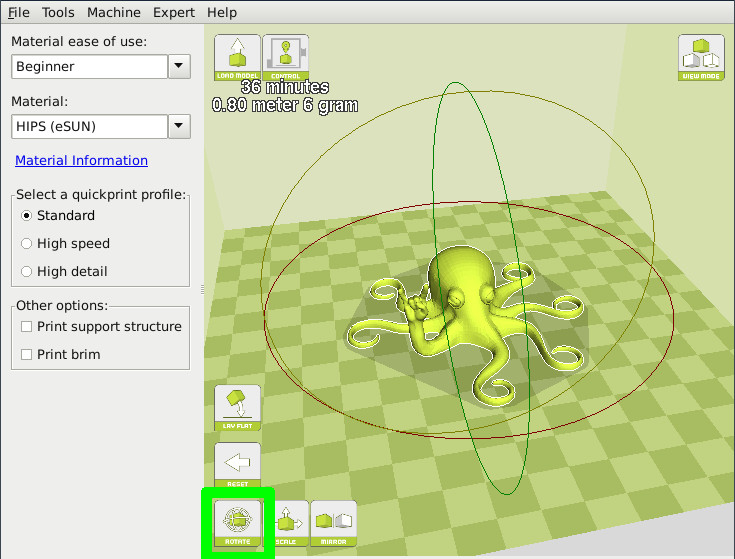
\includegraphics[keepaspectratio=true,angle=0,height=0.4\textheight,width=1.0\textwidth]{rotateoptions.jpg}
\caption{Rotating your Model}
\label{fig:Rotating your Model}
\end{figure}

\subsubsection{\texttt{Lay Flat}}
The \texttt{Lay Flat} button will ensure that the flat portion of your print is securely attached to the bed. It is highly recommended to use this option after rotating your model in the Z direction, as it will help prevent potential adhesion issues during the print.
%\begin{figure}[hbt]
%\centering
%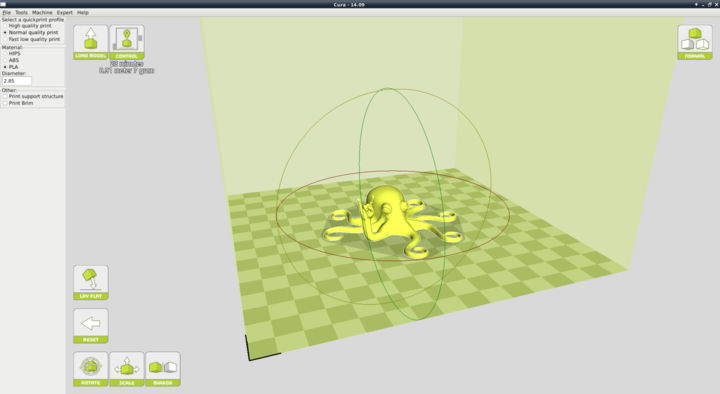
\includegraphics[keepaspectratio=true,angle=0,height=0.4\textheight,width=1.0\textwidth]{Rotate.png}
%\caption{Rotating your Model}
%\label{fig:Rotating your Model}
%\end{figure}

\subsubsection{\texttt{Reset}}
The \texttt{Reset} button will return your model to the original orientation as defined by the CAD program used to create the model.
%\begin{figure}[hbt]
%\centering
%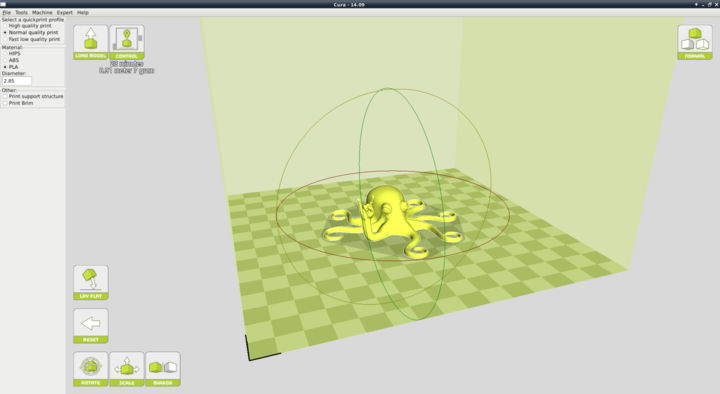
\includegraphics[keepaspectratio=true,angle=0,height=0.4\textheight,width=1.0\textwidth]{Rotate.png}
%\caption{Rotating your Model}
%\label{fig:Rotating your Model}
%\end{figure}

\subsubsection{\texttt{Scale}}
The \texttt{Scale} button displays the model dimensions, along with the ability to scale along the X Y or Z axes. Anything \texttt{below} the number \texttt{1.0} will reduce the objects size, while anything \texttt{above} the number \texttt{1.0} will increase the objects size. As a default, it will be set to uniform scaling. This will cause the X Y and Z axes to be scaled by the same amount when you make a change to any of them. To disable this, select the lock in the lower section of the scaling window. 
\begin{figure}[H]
\centering
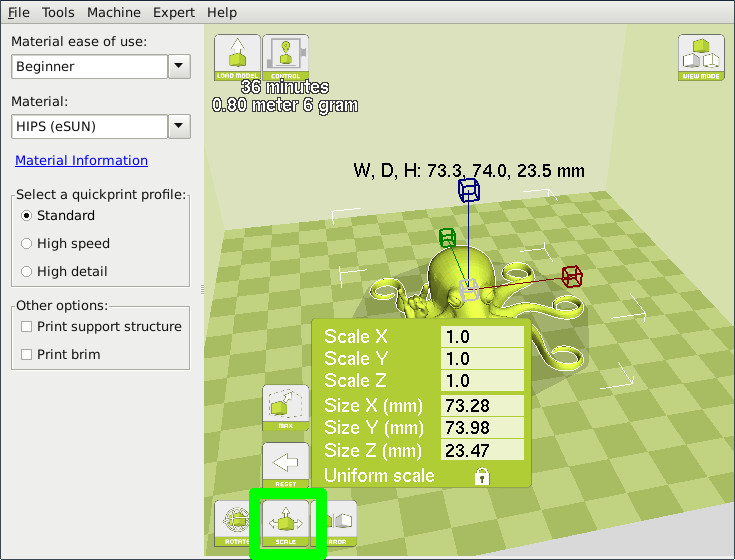
\includegraphics[keepaspectratio=true,angle=0,height=0.4\textheight,width=1.0\textwidth]{scaleoptions17.1.jpg}
\caption{Scaling your Model}
\label{fig:Scaling your Model}
\end{figure}

\section{\texttt{View Options}}
\index{View Options}
Different modes allow you to view your model in a variety of different ways. This can be helpful for spotting issues before the print even starts. 

\subsection{\texttt{Normal}}
\index{normal view}
This is the standard view and shows the solid outer surfaces of the model. (Fig. \ref{fig:Normal View}, page \pageref{fig:Normal View}): 

\begin{figure}[H]
\centering
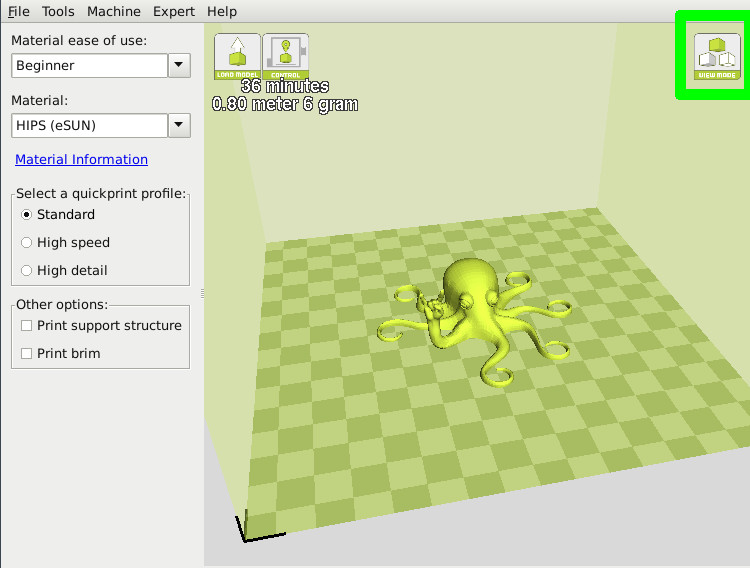
\includegraphics[keepaspectratio=true,angle=0,height=0.3\textheight,width=1.0\textwidth]{normalview17.1.jpg}
\caption{View in Normal Mode}
\label{fig:Normal View}
\end{figure}

\subsection{\texttt{Overhang}}
\index{Overhang} 
Overhang mode shows where your model may need support material. In Fig. \ref{fig:Overhang_View}, page \pageref{fig:Overhang_View} the red highlighted areas show overhangs and more severe angles and areas where support material is recommended. The overhang threshold can be defined in Expert Settings. 
\begin{figure}[H]
\centering
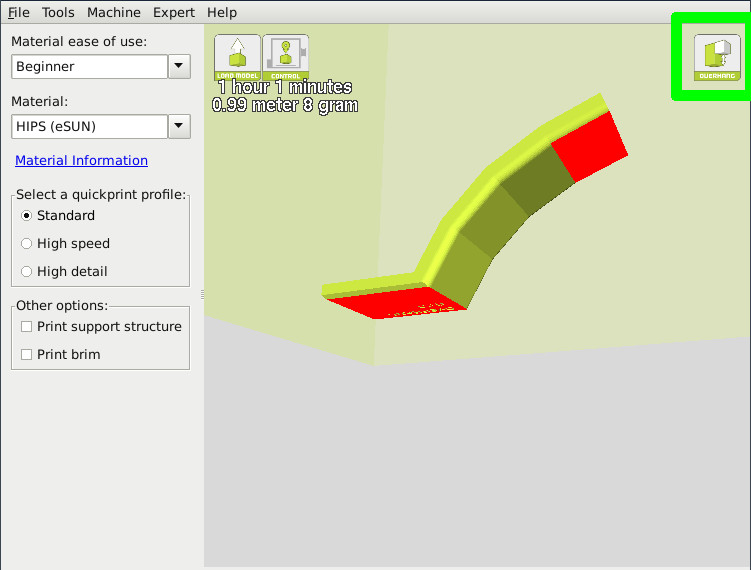
\includegraphics[keepaspectratio=true,angle=0,height=0.3\textheight,width=1.0\textwidth]{overhang17.1.jpg}
\caption{View in Overhang}
\label{fig:Overhang_View}
\end{figure}

\subsection{\texttt{Ghost}}
\index{Ghost}
Ghost view mode makes the model translucent to allow you to see what is behind it.
\begin{figure}[H]
\centering
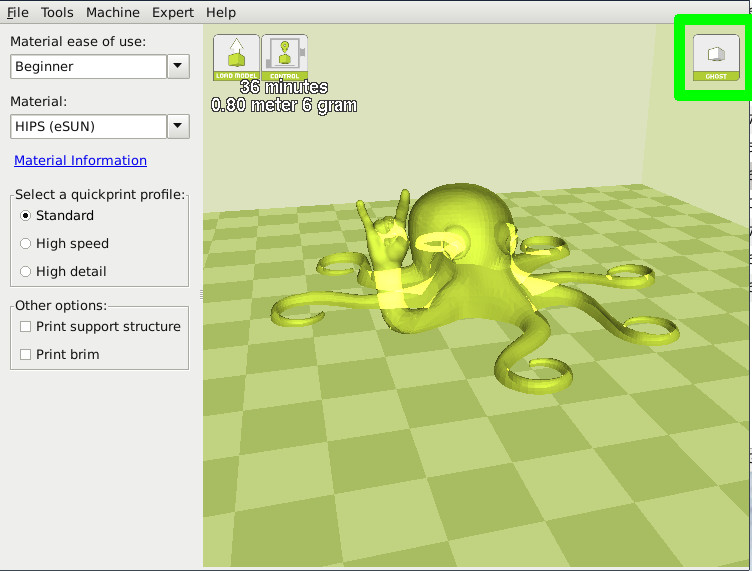
\includegraphics[keepaspectratio=true,angle=0,height=0.3\textheight,width=1.0\textwidth]{ghost17.1.jpg}
\caption{View in Ghost}
\label{fig:Ghost View}
\end{figure}

\subsection{\texttt{Xray}}
\index{Xray}
X-ray allows you to look inside of the object. This is helpful for detecting any manifold errors or other possible issues with your model. Problem areas will be highlighted in red. (Fig. \ref{fig:Xray View}, page \pageref{fig:Xray View})
\begin{figure}[H]
\centering
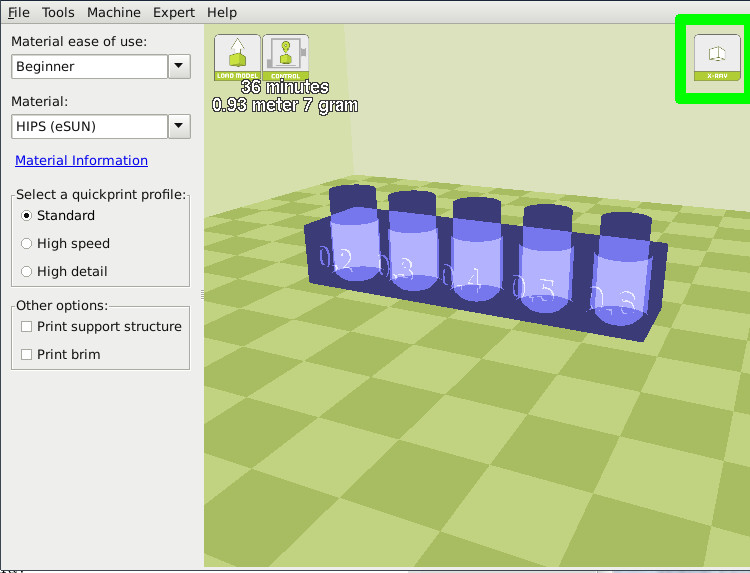
\includegraphics[keepaspectratio=true,angle=0,height=0.3\textheight,width=1.0\textwidth]{xray17.1.jpg}
\caption{View in Xray}
\label{fig:Xray View}
\end{figure}

\subsection{\texttt{Layers}}
\index{Layers}
To view the tool path of your print head and to ensure no skipped layers or gaps use this option. Use the slide bar on the right hand side of the window to move up and down through the tool path layers. Click the icon below it to view an individual layer at a time. If the \texttt{Print support structure} option is activated in Cura, support structure will be shown in blue.
\begin{figure}[H]
\centering
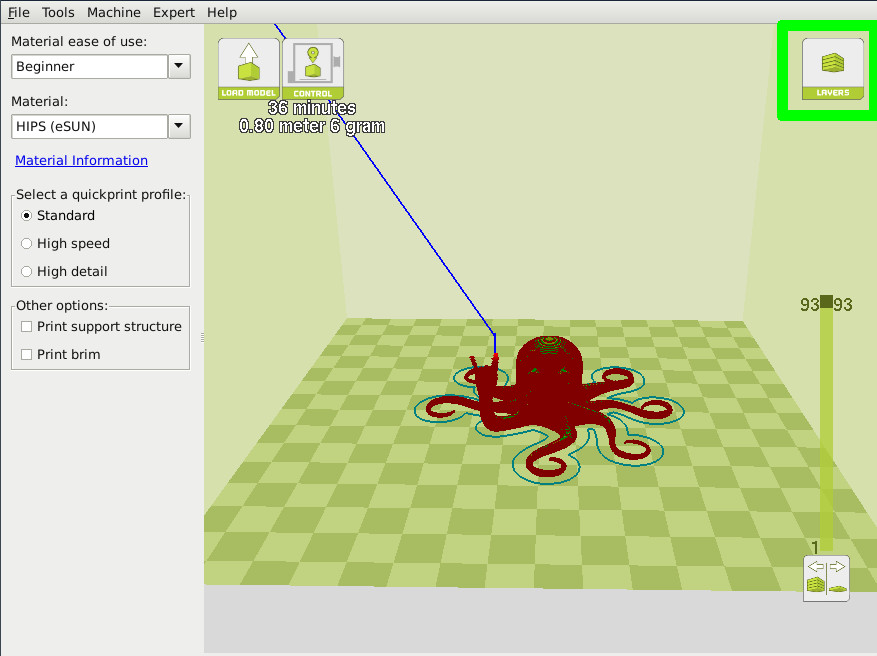
\includegraphics[keepaspectratio=true,angle=0,height=0.3\textheight,width=1.0\textwidth]{layers1.17.1.jpg}
\caption{View in Layers}
\label{fig:Layers View}
\end{figure}

\begin{figure}[H]
\centering
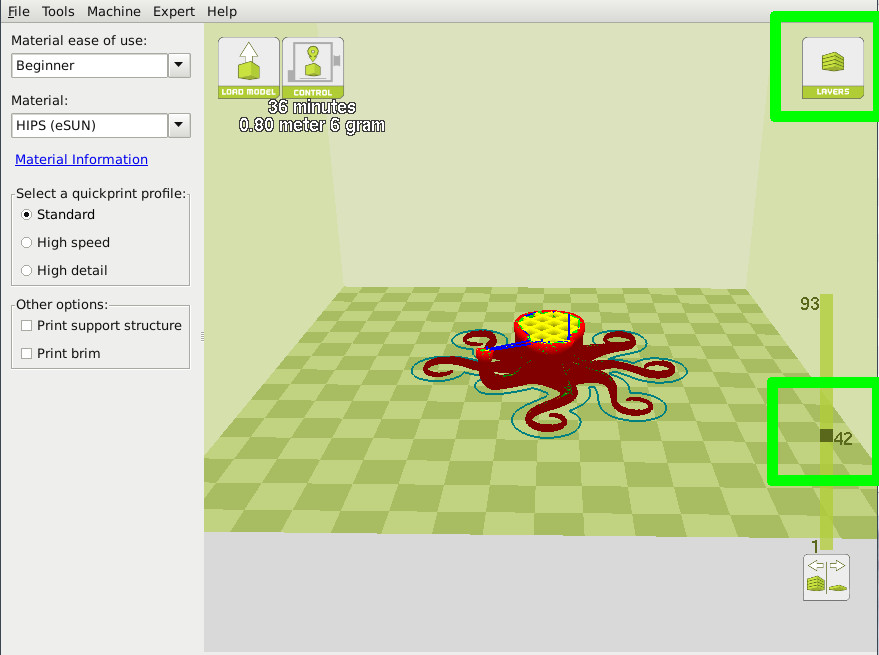
\includegraphics[keepaspectratio=true,angle=0,height=0.3\textheight,width=1.0\textwidth]{layers2.17.1.jpg}
\caption{Viewing Specific Layers}
\label{fig:Mid Layers View}
\end{figure}

\begin {figure}[H]
\centering
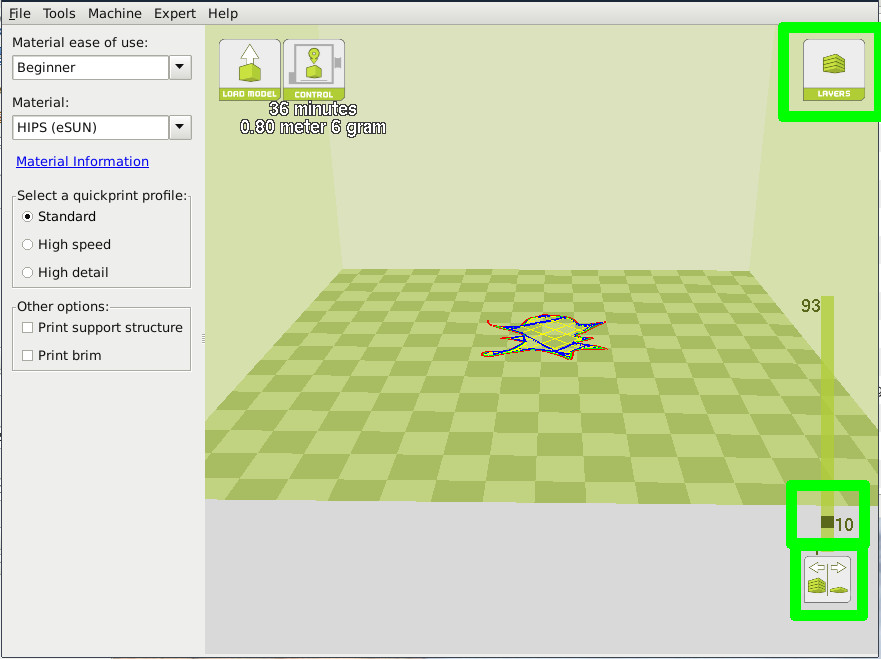
\includegraphics[keepaspectratio=true,angle=0,height=0.3\textheight,width=1.0\textwidth]{layers3.17.1.jpg}
\caption{Viewing Individual Layer}
\label{fig:Specific Layer}
\end{figure}

\section{\texttt{Starting Your First Print}}
\index{First Print}
Once you have your model, profile, and filament loaded, it is time for your first print! Refer to the \texttt{Quick Start Guide} included with your 3D printer. A PDF version is available at \texttt{LulzBot.com/downloads}.
 

\begin{comment} %%%% Turn the following on for standalone Cura manual %%%%
\subsection{Mini}

Select the \texttt{Print/Control} option in the top left hand corner of your build volume. This will bring up your Pronterface user interface. Please wait for the window to state \texttt{operational} before sending any commands to the printer..

%\pageref{fig:Print Control}).
\begin{figure}[hbt]
\centering
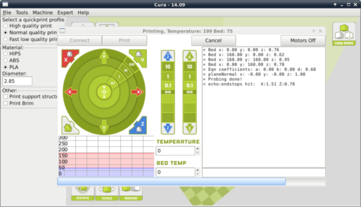
\includegraphics[keepaspectratio=true,angle=0,height=0.4\textheight,width=1.0\textwidth]{print_control.png}
\caption{Print Control Screen}
\label{fig:Print Control}
\end{figure}

\subsection{TAZ}

TAZ users will need to decide if they want to print directly from their computer using the USB cable, or if they would like to print from their SD card.

%%%% SD Printing %%%%
\subsubsection{Printing from SD Card}
\index{Printing from SD}

Save your Gcode file to your SD card. Select \texttt{File} > \texttt{Save Gcode} and choose the SD card location. Insert the SD Card into the Graphical LCD Controller.

\subsection{Set Temperature}

Turn on the heated bed and hot end by using the Graphical LCD controller and navigating to: \texttt{Prepare} > \texttt{Preheat ABS or PLA}. If you are using other materials you can set your desired temperatures by going to \texttt{Control} > \texttt{Temperature} > \texttt{Nozzle/Bed}. Wait for your 3D printer to reach specified temperatures.

\subsection{Start Print}
\index{printing}
Once at the desired printing temperature begin your print through your Graphical LCD controller by navigating to: \texttt{Print From SD} > and select the desired file.

%%%% Tethered printing %%%%

\subsubsection{Printing from USB Cable}
\index{Printing from USB}

Connect your 3D printer using a USB cable and select the \texttt{Print/Control} button. This will bring up the Pronterface user interface. You will not be able to send any commands until the window title changes to \texttt{Operational}. 

\subsubsection{Set Temperature}

Set your temperatures for the hot end and the bed. You will see two boxes, one labeled “Temperature” and one labeled “Bed Temp”. Temperature will set your hot end, and bed temp will set your bed. Once your hot end and bed have reached temperature, you will just need to select print.

\end{comment} 

\subsection{\texttt{Printing from USB Cable}}
\index{printing from USB}
\index{USB}
\index{USB cable}
Connect your 3D printer to a computer using a USB cable, power it on and select the \texttt{Control} button at the top of the 3D viewing window. If the control button is not present, be sure you have a model file loaded into Cura. If a model is loaded but the Control button is still not present use a different USB port, reinstall Cura, or contact our Support Team. This will bring up your Printer Interface. You will not be able to send any commands until the window title changes to \texttt{Operational}. Once operational, you can start your first print. Your Mini will then go through it's automatic cleaning and wiping process before starting the print. This should take approximately 5 minutes.

%\pageref{fig:Print Control}).

\begin{figure}[H]
\centering
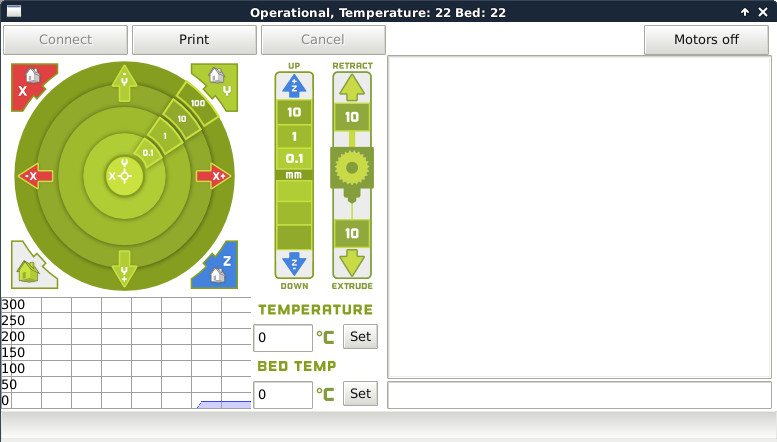
\includegraphics[keepaspectratio=true,angle=0,height=0.4\textheight,width=1.0\textwidth]{ControlBox17.1.jpg}
\caption{Control Screen}
\label{fig:Control}
\end{figure}
\subsection{\texttt{Pausing Mid-Print}}
\index{pausing in the printing process}
\index{pause print}
You will notice after you click the print button through Cura, it will change to a pause button. When activated, it will pause your print and automatically move your print head away from your object. This will allow color changes or material changes mid print.

\subsection{\texttt{Automatic Bed Leveling}}
\index{automatic bed leveling}
\index{ABL}
Before each print your Mini will go through a wiping and a probing procedure in order to determine the slope/tilt of your bed. If your nozzle is dirty or not cleaned properly, this will prevent the printer from being able to create an electrical contact with the corners. Your Mini will automatically retry the wiping and probing procedure if this happens, up to a maximum of three times. If three consecutive wipes and probes have failed, the printer will stop and a warning will sound. If this is happening consistently, you should replace the wiping pad and/or adjust your wiping and probing temps for that specific filament. See section \ref{sssec:num1} on page \pageref{sssec:num1} for details on changing these temps.

\subsection{\texttt{Recommended Temperatures}}
\index{Temperatures}
Different filaments have different ideal temperatures for extrusion, bed adhesion, and part removal. Your LulzBot Mini will have these automatically set when using our recommended profiles. We have found that for certain materials a glue stick is required for successful bed adhesion and/or part release. Glue stick can also be added to help first layer adhesion on any material, and may be helpful for objects with a larger surface area. 
\begin{table}[H]
	\begin{center}
 		\hspace*{-1.5cm}\begin{tabular}{||c c c c c||} 
 		\hline
 		Filament Type & Bed Preparation & Nozzle Temp & Bed Temp & Removal Temp \\ [0.5ex] 
 		\hline\hline
 		ABS & Clean PEI & 230-250 & 110 & 50 \\ 
 		\hline
 		PLA & Clean PEI & 195-215 & 60 & 45\\
 		\hline
 		HIPS & Clean PEI & 230-250 & 110 & 50 \\
 		\hline
 		Laywoo-D3 & Clean PEI & 175-195 & 60 & 45 \\
 		\hline
		bambooFill & Clean PEI & 185-195 & 60 & 50 \\ 
 		\hline
		woodFill & Clean PEI & 185-195 & 60 & 50 \\
 		\hline
 		Laybrick & Clean PEI & 175-195 & 60 & 45 \\
		\hline
		bronzeFill & Clean PEI & 225-235 & 60 & 50 \\
		\hline
		copperFill & Clean PEI & 225-235 & 60 & 50 \\
 		\hline 
 		Magnetic Iron PLA & Clean PEI & 220-230 & 60 & 50 \\
 		\hline
 		Stainless Steel PLA & Clean PEI & 220-230 & 60 & 50 \\
 		\hline
 		Conductive PLA & Clean PEI & 215-230 & 60 & 50 \\
		\hline
		High Temp PLA & Clean PEI & 220-230 & 60 & 40 \\
 		\hline
 		nGen & Clean PEI & 220-240 & 85 & 60 \\
 		\hline
 		t-glase & Glue stick & 240-260 & 60 & 45 \\
 		\hline
 		Flexible Filaments & Glue stick & 215-230 & 50 & 35 \\  
 		\hline
 		Nylons & Glue stick & 220-270 & 110 & 50 \\
 		\hline
 		Polycarbonate & Glue stick & 260-300 & 110 & 50 \\ 
 		\hline
 		Polycarbonate + ABS & Glue stick & 260-280 & 110 & 50 \\
 		\hline
 		INOVA 1800 & Glue stick & 235-255 & 75 & 50 \\
 		\hline
 		n-vent & Glue stick & 225-245 & 60 & 50 \\ [1ex]
 		\hline
 
		\end{tabular}
		\caption{Recommended Temperatures}\label{tab:a}
	\end{center}
\end{table}
 


\section{\texttt{Removing Your First Print}}
\index{Removing a Print}
After your first print has finished, you need to wait for the part to cool down.  Your parts will be easier to remove if you allow your heated bed to cool down to optimal temperature. This will allow the plastic to contract, making it easier to remove. \texttt{Your print bed will move forward once it is ready to be removed.}

Once your heated bed has cooled, use the blue handled knife that was included with your printer to remove the item. Carefully insert the blade of the knife between your print and heated bed. Once underneath the part rotate the blade- lifting with the sharp edge into the part, to gently pop the piece off your plate.
%\begin{figure}[hbt]
%\centering
%\includegraphics[keepaspectratio=true,angle=0,height=0.4\textheight,width=1.0\textwidth]{remove_part.png} %%%% Photo needed %%%%
%\caption{Remove Part}
%\label{fig:Remove part}
%\end{figure}

\section{\texttt{Full Settings}}
\index{Full Settings}
When you first switch to Full Settings, Cura will need to know what filament, manufacturer, and quality you wish to use. It will automatically transfer our quickprint settings over to allow adjustments if one is selected. \textcolor{red}{IF A QUICKPRINT PROFILE IS NOT AVAILABLE, YOU WILL NEED TO MANUALLY LOAD ONE IN.} We recommend using our tested profiles that are available here: \texttt{https://www.lulzbot.com/cura}. You will want to choose the profile that matches your filament and quality needs. Once downloaded, you can load the file into Cura by selecting \texttt{File} > \texttt{Open Profile}. This will automatically update all of your Cura settings for use with your specific filament.
\begin{figure}[H]
\centering
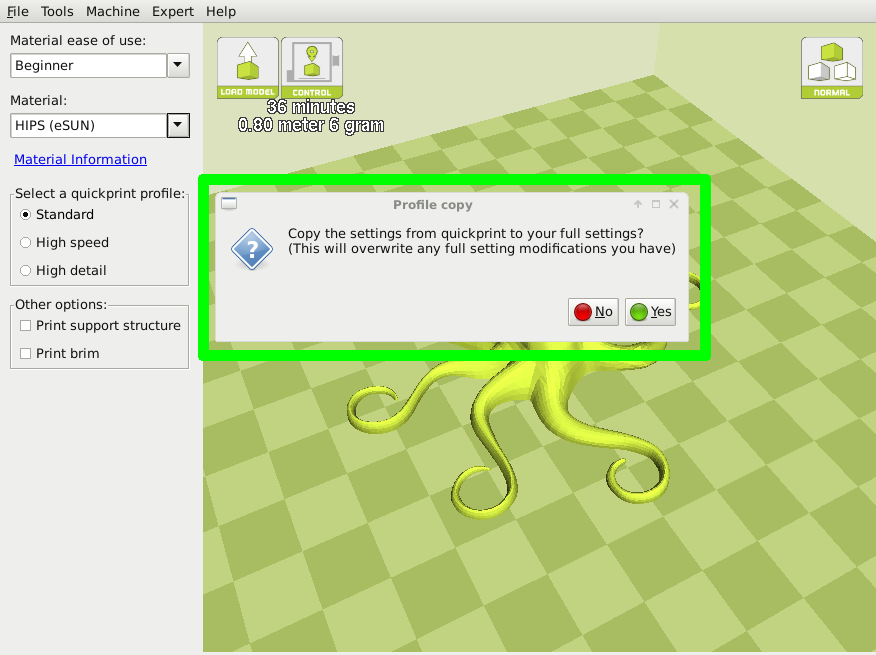
\includegraphics[keepaspectratio=true,angle=0,height=0.4\textheight,width=1.0\textwidth]{copyprofile.jpg}
\caption{Transferring a Profile}
\label{fig:Transferring a Profile}
\end{figure}
Once the switch has been made to full settings, you will now have access to a wide variety of options. You will notice 4 new tabs: \texttt{Basic, Advanced, Plugins, Start/End-Gcode}. In the following sections we will describe each option, and how they will affect your prints.
\begin{figure}[H]
\centering
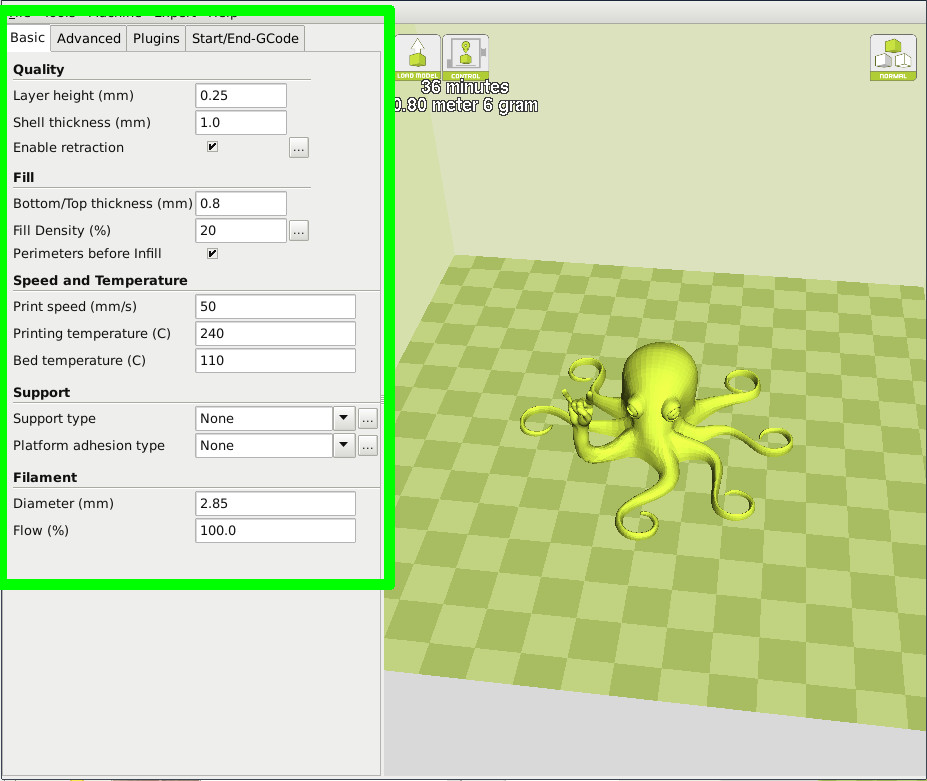
\includegraphics[keepaspectratio=true,angle=0,height=0.4\textheight,width=1.0\textwidth]{fullsettings17.1.jpg}
\caption{View in Full Settings}
\label{fig:View in Full Settings}
\end{figure}

%\subsection{\texttt{Loading a Profile}}
%\index{Loading Profile}
%Profiles determine how Cura turns your STL file into Gcode that controls your printer. Different filaments require different settings for optimal performance. As new filaments are being developed every day, there may be a time you need to manually load a profile. You can download our recommend profiles at: \texttt{https://www.lulzbot.com/support/mini-cura-profiles}. Once downloaded, load the filament specific .ini file by going to \texttt{File > Open Profile}.
%\begin{figure}[hbt]
%\centering
%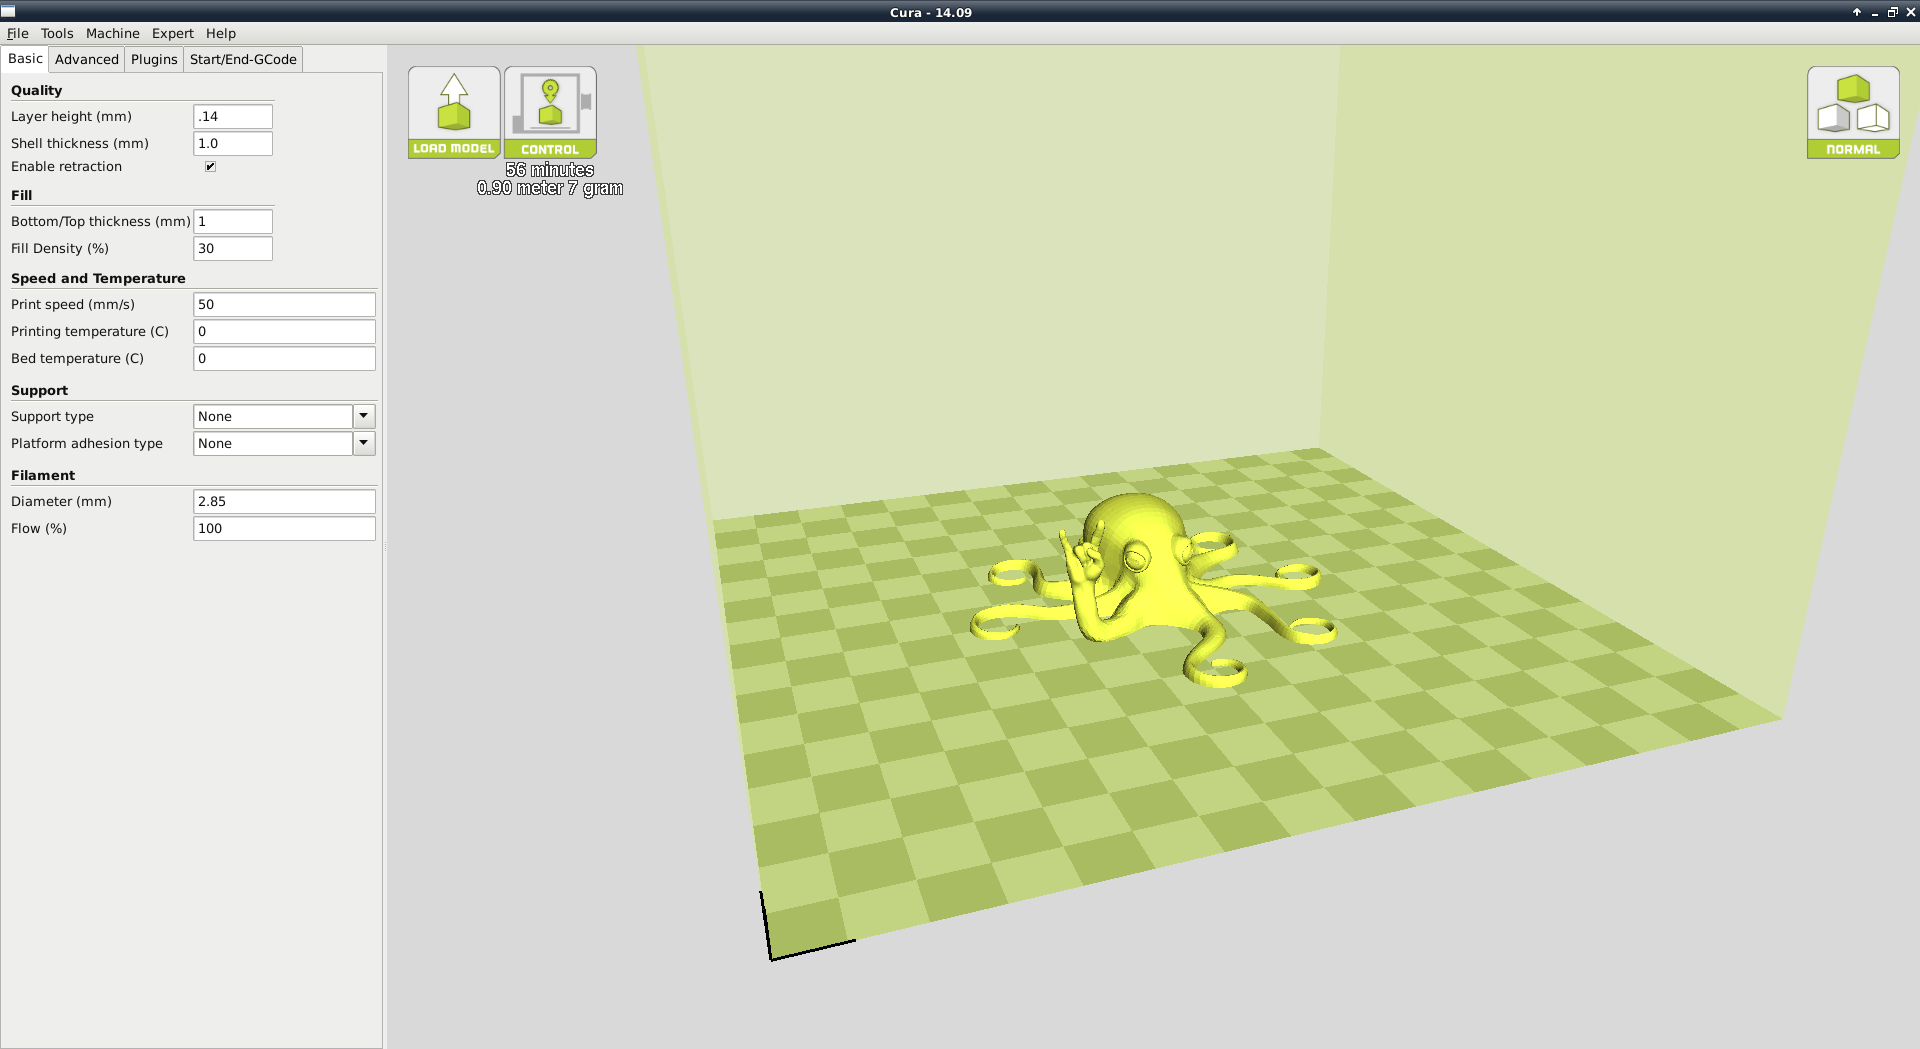
\includegraphics[keepaspectratio=true,angle=0,height=0.4\textheight,width=1.0\textwidth]{Expert.png}
%\caption{View in Full Settings}
%\label{fig:Full Settings View}
%\end{figure}

\section{\texttt{Basic Tab Options}}
\index{Basic Options}

\subsubsection{\texttt{Layer Height}}
\index{Layer Height}
The thickness of each printed layer is known as the ``Layer Height''. The smaller the layer height, the smoother curves will appear. Larger layer heights are better for bridging and overhangs. Smaller layer heights will also increase print time, as it will take more layers to complete the object.
% (Layer height comparision photos)
\begin{figure}[H]
\centering
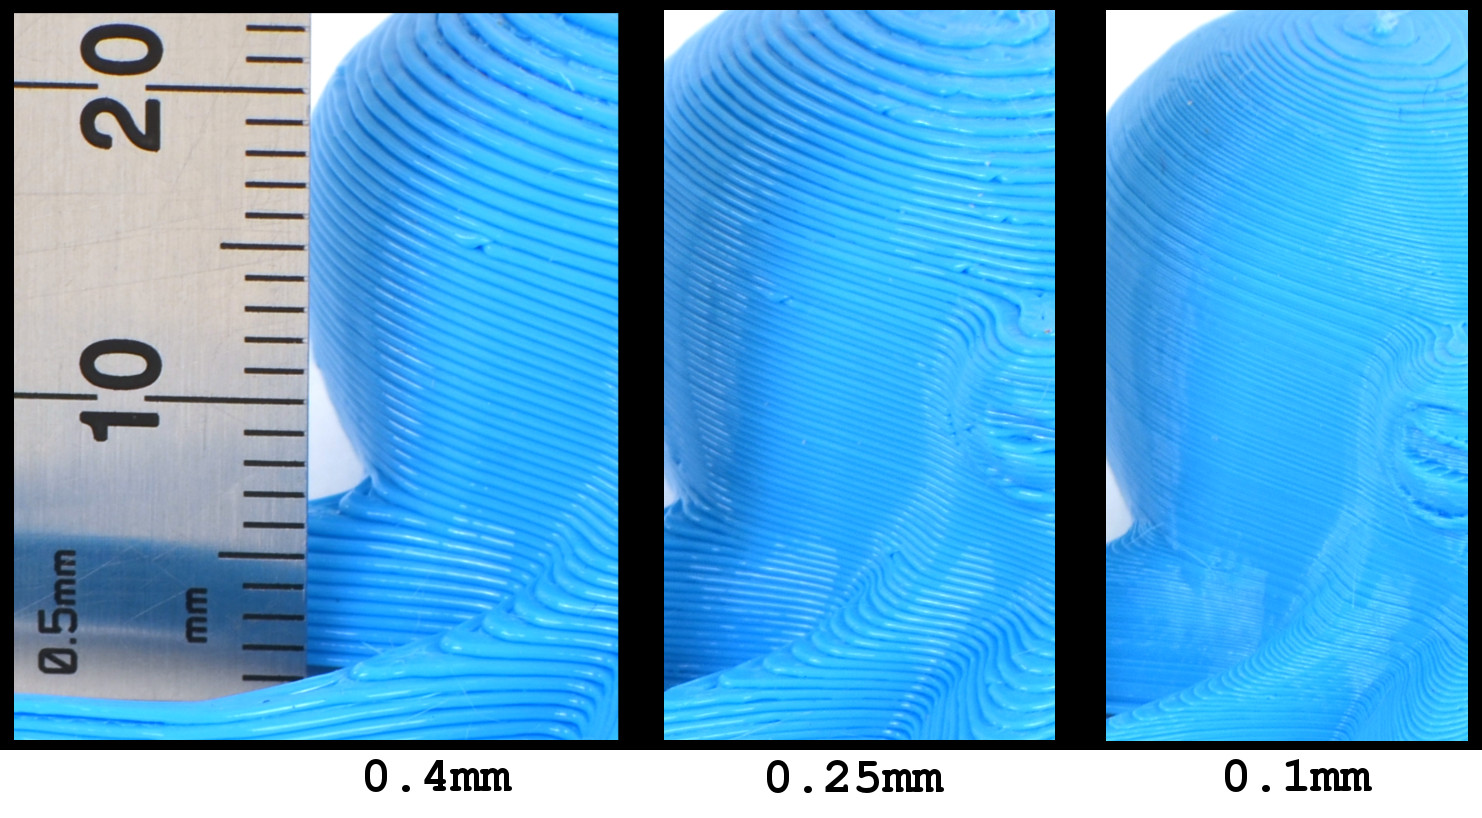
\includegraphics[keepaspectratio=true,angle=0,height=0.4\textheight,width=1.0\textwidth]{ManualLayerHeight.jpg}
\caption{Differences in Layer Height}
\label{fig:Differences in Layer Height}
\end{figure}


\subsubsection{\texttt{Shell Thickness}}
\index{Shell Thickness}
This defines the number of vertical walls that comprise the outside of your model. We recommend keeping this set to multiples of your nozzle width. Your LulzBot Mini 3D printer is equipped with a 0.5mm nozzle. A setting of 1.0mm or 1.5mm is a sufficient for most prints.

\subsubsection{\texttt{Enable Retraction}}
\index{Retraction}
Retraction tells your printer to pull filament out of the hot end upon travel moves. Travel moves are when your print head moves from one area of the print, to another without laying down filament. We recommend keeping this on for all filament types, and adjusting the retraction length and speed for the specific filament.
%(Details given in advanced tab section. ((Reference?))

\subsubsection{\texttt{Bottom/Top Thickness (mm)}}
\index{Bottom Thickness}
\index{Top Thickness}
Also known as ``Surface Layers'' this will determine how thick the top and bottom layers are. A larger number here will create a thicker top and bottom which can be helpful for strength, bridging, and quality purposes. We recommend keeping this number as a multiple of your layer height.

\subsubsection{\texttt{Fill Density}}
\index{Fill Density}
This number is expressed as a percentage. 0\% will give a completely hollow print, while 100\% will give you a completely solid object. We have found that 20\% to 40\% fill density is functional for most prints.

\subsubsection{\texttt{Perimeters Before Infill}}
This option will toggle the order in which the infill and perimeters will be printed. We recommend leaving this on.

\subsubsection{\texttt{Print Speed (mm/s)}}
\index{Print Speed}
Your overall printing speed can be adjusted here. This setting will be overridden in certain parts of the print based upon your Advanced Speed Settings. If no speeds are determined in the advanced settings tab, your printer will default to this setting. %See Advanced Section \ref{sssec:Travel Speed}, page \pageref{sssec:Travel Speed} 


\subsubsection{\texttt{Printing Temperature}}
This is where you will set the hot end temperature for your specific material and manufacturer. It will be preset when using the recommended quickprint profiles. This can be adjusted for fine tuning of different filament manufacturers to help layer adhesion or stringing. \texttt{See Recommended Temperatures Table: page \pageref{tab:a}.} Your hot end is capable of reaching a maximum temperature of \texttt{300°C}.

%%%% Since the Mini needs to have gcode temps set in order to run through auto bed leveling, the following statement is only applicable to the TAZ4 or earlier. %%%%
%We recommend leaving this temperature setting to “0”. If you set your temperature in this section your printer will not begin printing until it reaches the specified temperature. We recommend setting your printing temperatures through the Pronterface UI, or through your LCD.

\subsubsection{\texttt{Bed Temperature}}
\index{bed temperature}
This is where you will set the print surface temperature for your specific material. These will be preset when using the recommended quickprint profiles. This can be adjusted for fine tuning of different filament manufacturers to help adhesion or release. \texttt{See Recommended Temperatures Table: page \pageref{tab:a}.} Your print surface is capable of reaching a maximum temperature of \texttt{135°C}. 

\subsection{\texttt{Support Type}}
\index{Support Type}
Some models will require support material in order to print properly. This will usually occur when an object has an angle in relation to the build plate between 0 to 45 degrees. It is highly recommended to orient or design your object so that it minimizes or eliminates the need for support.

\subsubsection{\texttt{Touching Buildplate}}
This causes the support material to build up between the heated bed and the object. The red example is Touching Buildplate. (Fig. \ref{fig:Different Types of Support}, page \pageref{fig:Different Types of Support}) 
% (Photo of Circle inside a square, that is printed vertically. Have samples on photo table. Reference photo below?)

\subsubsection{\texttt{Everywhere}}
This prints support material between the heated bed and object as well as between the object and itself. The green example is Support Everywhere. (Fig. \ref{fig:Different Types of Support}, page \pageref{fig:Different Types of Support})
% (Photo of Circle inside a square, that is printed vertically, sample on photo table. Reference Photo Below?)
% (Support Comparison Photo)
\begin{figure}[H]
\centering
\includegraphics[keepaspectratio=true,angle=0,height=0.4\textheight,width=1.0\textwidth]{Support_Revised.jpg}
\caption{Support Types}
\label{fig:Different Types of Support}
\end{figure}

\subsection{\texttt{Platform Adhesion Type}}
\index{Adhesion Type}
Some models have a small surface area contacting the plate. This can create adhesion issues causing your part to pop off at some point during the print. To fix this, use either \texttt{Brim} or \texttt{Raft}. Raft is better used when a model has small heated bed contact points and overhangs.

\subsubsection{\texttt{Brim}}
\index{Brim}
Brim will create a single layer of filament, contacting and surrounding your model. This will increase the surface area of the part contacting the build platform thereby preventing it from popping off the heated bed. Brim will also help in situations where you are seeing corner lift. Brim settings can be adjusted in the \texttt{Expert Settings} options. %See Expert Settings \ref{sssec:Brim Line Amount}, page \pageref{sssec:Brim Line Amount} 
% (See Expert Settings/Page REFERENCE)

\subsubsection{\texttt{Raft}}
\index{Raft}
%% Raft is rarely used these days %%
Raft will generate a layer (or more) of material underneath your object. Raft was more often used before the addition of heated plates to increase surface area and reduce warp. Raft settings can be adjusted in the \texttt{Expert Settings} options.

\subsection{\texttt{Filament Diameter}}
\index{Filament Diameter}
The filament diameter setting is one of the more important settings. Make sure that you update this value periodically with your average filament diameter. While your filament may be referred to as 3mm, it is more likely going to be near 2.85mm +/- 0.1mm. You will want this to be an accurate average, as it will allow your printer to correctly calculate how much filament it is pulling into the hot end. The default value should be set to 2.85mm.

\subsection{\texttt{Filament Flow \%}}
\index{Flow Rate}
This controls how much filament your printer is extruding in relation to speed. This setting is mainly used to adjust for filament density variations. This may need to be changed when switching between different manufacturers or types of filament to adjust for die swell. It is recommended to make small adjustments between prints for fine tuning.

\section{\texttt{Advanced Tab Options}}
\index{Advanced Options}
\begin{figure}[H]
\centering
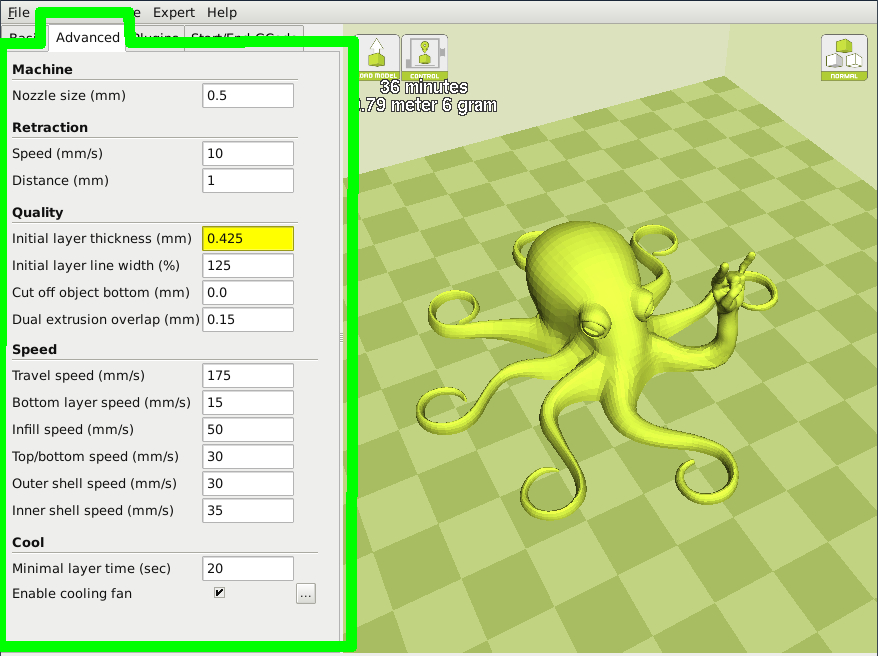
\includegraphics[keepaspectratio=true,angle=0,height=0.4\textheight,width=1.0\textwidth]{advanced.jpg}
\caption{View of Advanced Tab}
\label{fig:View of Advanced Tab}
\end{figure}

\subsection{\texttt{Nozzle Size (mm)}}
\index{Nozzle Size}
%%%% standalone version line %%%%
%This defines your nozzle size. The slicing engine uses this value combined with your other settings to determine how quickly to feed filament into your hot end. The TAZ ships with a 0.35mm nozzle, and the TAZ Mini ships with a 0.5mm nozzle.
This defines your nozzle size. The slicing engine uses this value combined with your other settings to determine how quickly to feed filament into your hot end, and how to generate the tool path. The LulzBot Mini ships with a 0.5mm nozzle standard.

\subsection{\texttt{Retraction Speed (mm/s)}}
\index{Retraction Speed}
Retraction Speed determines the speed at which your filament is reversed out of the hot end for travel moves and when changing direction during printing. We recommend keeping this set to less than 25mm/s to help protect the gears.

\subsection{\texttt{Retraction Distance}}
\index{Retraction Distance}
Retraction Distance determines how much filament is pulled out of your hot end on travel moves and when changing direction. You will want to adjust this depending on temperature settings and filament type. Higher thermal retaining filaments such as PLA behave better with a longer retraction distance. We have found anywhere from 1mm to 3mm is a good starting range.
% changed from "1 to 6mm" to remain conservative.

\subsection{\texttt{Initial Layer Thickness}}
\index{Initial Layer}
This will control how thick your first printed layer height is printed onto the heated bed. A larger initial layer height is more forgiving and will help first layer adhesion. All of our standard profiles have a 0.425mm initial layer height. This eliminates the need for adjustments when switching between filaments.  \textcolor{red}{Your LulzBot Mini automatic bed leveling system could be affected if you change this from the standard profiles. Adjust at your own risk.} If you want to change first layer "squish" see Z Offset \ref{sssec:Z Offset}, page \pageref{sssec:Z Offset} 

\subsection{\texttt{Initial Layer Line Width}}
\index{Initial Layer Width}
This will control how wide your first extruded filament path is for the initial layer. A wider line width will help with bed adhesion. We have found 125\% to be a good starting place. For models with moving, printed in place parts, a smaller initial layer line width is recommended. \textcolor{red}{Your LulzBot Mini automatic bed leveling system could be affected if you change this from the standard profiles. Adjust at your own risk.} If you want to change how much your first few layers "squish" to the sides, see Z Offset \ref{sssec:Z Offset}, page \pageref{sssec:Z Offset} 


\subsection{\texttt{Cut Off Object Bottom (mm)}}
\index{Cut Off Object}
This setting is used to help print models that were not specifically designed for FFF printing. Specifically, it is for models that do not have a flat surface to adhere to the plate. It will sink your object Xmm into the build plate, creating a nice flat surface to begin your print. You can also use this option to remove the lower portion of your model.
\begin{figure}[H]
\centering
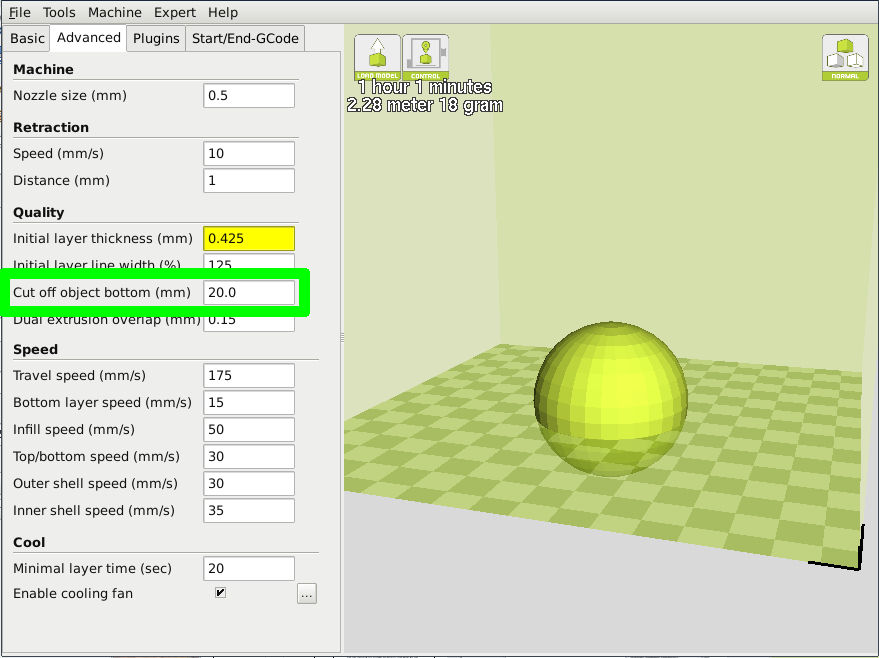
\includegraphics[keepaspectratio=true,angle=0,height=0.4\textheight,width=1.0\textwidth]{cutoff17.1.jpg}
\caption{Cutoff Example}
\label{fig:Cutoff Example}
\end{figure}

\subsection{\texttt{Dual Extrusion Overlap}}
\index{Dual Extrusion Overlap}
This will determine how far your Dual Extruders will overlap when laying down material. This will help adhesion between the two different colors or types of filament. This setting is only used when the printer is equipped with two hot ends and extruders.

\subsection{\texttt{Travel Speed}}
\index{Travel Speed}
This setting will determine how fast your print head moves while not extruding filament. A normal travel speed of 125 - 150mm/s is recommended.

\subsection{\texttt{Bottom Layer Speed}}
\index{Bottom Layer Speed}
This will control your initial layer speed. In general, a slower initial layer speed will help with first layer adhesion. 

\subsection{\texttt{Infill Speed}}
\index{Infill Speed}
This is how fast your print head speed will be while laying down the interior portion of your model. Faster speeds are usually tolerable here, as none of the infill will be visible from the outside of your object. If you go too fast compared to your inner and outer shells, you can have adhesion issues or globs of filament left behind from the printhead.

\subsection{\texttt{Outer Shell Speed}}
\index{Outer Shell Speed}
This will be the outermost surface of the model. This is the most important setting, as it controls the speed of your print head on the visible layers. As a general rule of thumb, the slower you go the better looking print you will get. 

\subsection{\texttt{Inner Shell Speed}}
\index{Inner Shell Speed}
This affects vertical walls that are in between the outer shell and infill. This will not be visible but will help support the outer shell and the infill. We recommend keeping this speed setting between your infill and your outer shell speed.

\subsection{\texttt{Minimal Layer Time}}
\index{Minimal Layer Time}
This will determine a minimum amount of time your printer will spend laying down each layer. If your layer print time falls below this your printer will automatically slow down to reach this time before moving onto the next layer. Tweaking this can help get cleaner, crisper prints.

\subsection{\texttt{Enable Cooling Fan}}
\index{Enabling Cooling Fan}
Enables operation of your extruder's active cooling fan. The fan settings can be adjusted in the \texttt{Expert Settings} options.

\section{\texttt{Plugins}}
\index{Plugins}
Plugins are custom settings which will alter your print at specific points. The two that come pre-loaded with Cura are \texttt{Tweak at Z}, and \texttt{Pause at Height}. More plugins and information can be found here: \texttt{http://wiki.ultimaker.com/Category:CuraPlugin} To activate one of these highlight the desired plugin and click the drop-down arrow directly below the Plugins box. 
\begin{figure}[H]
\centering
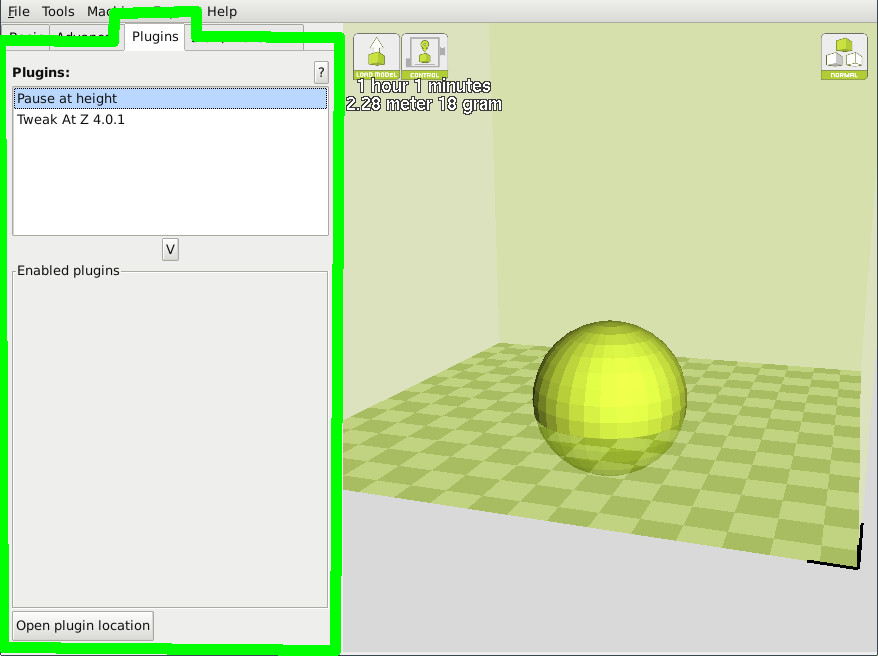
\includegraphics[keepaspectratio=true,angle=0,height=0.4\textheight,width=1.0\textwidth]{plugins17.1.jpg}
\caption{View of Plugins}
\label{fig:Plugins}
\end{figure}

\subsection{\texttt{Tweak at Z}}
\index{Tweak at Z}
Make basic changes at specified Z heights. You can determine the Z height or layer count at which you want to make a change. Then choose how you would like to change your settings. You can alter temperatures, fan speeds, and print speeds. Fine tuning these for specific STL files, can produce cleaner prints.

\subsection{\texttt{Pause at Z Height}}
\index{Pause at Z Height}
Pause your print at a specified height. You can also specify where to move the print head and how much filament to retract. This will prevent “blobs” from accumulating on your print while paused. This setting is most commonly used when switching colors of filaments in the middle of a print.

\section{\texttt{Start and End Gcode Settings}}
\index{Custom Gcode}
Custom Gcode allows for complex automatic printer movements and operations. By adding custom Gcode into the start or end of your file, you can alter how it prints. A comprehensive list of Gcode commands can be found here: \texttt{http://reprap.org/wiki/G-code} We recommend new users to leave this as provided in the profiles at \texttt{https://www.lulzbot.com/support/downloads}

\subsection{\texttt{Mini Specific Considerations}}
Please be cautious when changing any of these start and end gcode settings. \textcolor{red}{This is where your Auto Bed Leveling commands are stored. If improperly altered, your printer will no longer automatically compensate for the heated bed position and can even potentially damage components on the printer.} If you are uncertain of the change you are trying to make, please contact us at \texttt{Support@LulzBot.com} before hand.

\definecolor{green2}{rgb}{0.00,0.375,0.0}

\subsection{\texttt{Changing Wiping and Probing Temperatures}} \label{sssec:num1}
\index{wiping temperature}
\index{probing temperature}
We have set wiping and probing temperatures that we have found work well with specific types of filament and filament manufacturers. \texttt{If you are using a type and/or manufacturer of filament not listed in the quickprint settings, you may need to adjust these temperatures for optimal probing.} In the start GCODE section, there will be three separate temperatures you can adjust. What these GCODE lines do will be described in the \textcolor{green2}{green text} to the right of the command. The ones you will want to adjust are:
\begin{itemize}
\item \texttt{M109 SXXX}                    \textcolor{green2}{; soften filament for z homing}
\item \texttt{M104 SYYY}                    \textcolor{green2}{; wipe temp}
\item \texttt{M109 SZZZ}                    \textcolor{green2}{; heat to probe temp}
\end{itemize}

By changing the variables \texttt{(XXX, YYY, ZZZ),} you can change what temperature your printer will soften, wipe, and probe. Our temperatures for softening, wiping, and probing will be a good starting point for other manufacturer's filament. When making adjustments, we recommend \texttt{+/- 5°C} changes at a time. \texttt{Be sure to watch the probing sequence when experimenting with new temperatures.}

\section{\texttt{Expert Settings}}
\index{Expert Settings}
Expert settings will give you more specific options for your retraction, skirt, active cooling, infill, support, brim, raft, and special settings. To gain access to this section you go to \texttt{Expert} > \texttt{Open Full Settings} or on your keyboard press \texttt{Control + E}.
\begin{figure}[H]
\centering
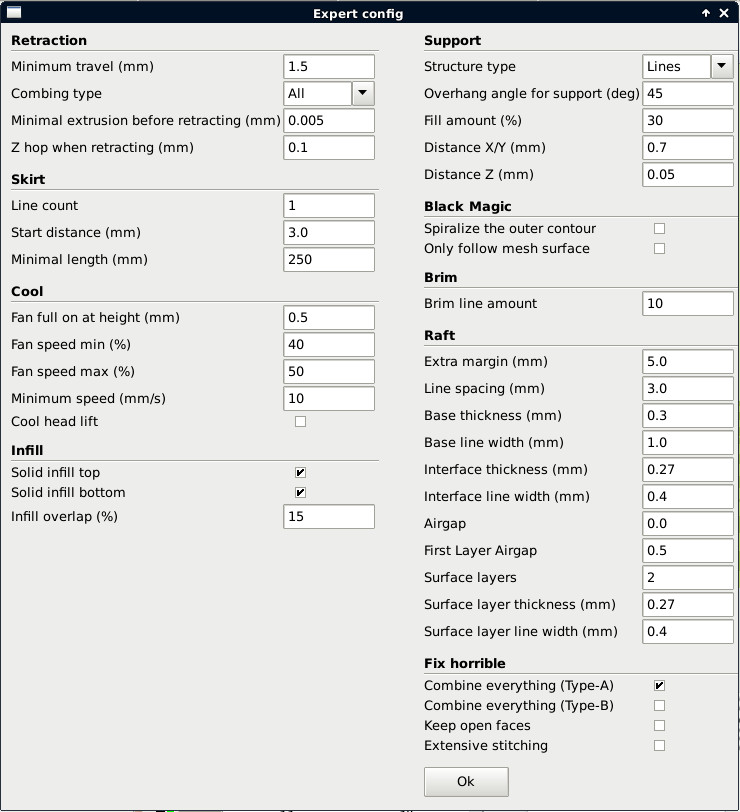
\includegraphics[keepaspectratio=true,angle=0,height=0.4\textheight,width=1.0\textwidth]{expert17.1.jpg}
\caption{View Expert Settings}
\label{fig:Expert Settings}
\end{figure}

\section{\texttt{Retraction}}
\index{Retraction}
Retraction pulls filament out of your nozzle when it is not extruding to prevent your print head from dripping on your object. This section is where you will control how your extruder retracts its filament.

\subsection{\texttt{Minimum Travel}}
\index{Minimum Travel}
This sets the minimum travel distance of your printhead in order to retract. If your print head is not moving this far during travel moves, it will not retract.

\subsection{\texttt{Combing}}
\index{Combing}
This option prevents your print head from traveling over holes in the X/Y plane when printing. This will slightly increase print time, but will prevent strings from getting caught on the holes during travel moves. We recommend keeping this setting on.

\subsection{\texttt{Minimal Extrusion Before Retracting}}
This will control the distance at which retraction occurs if the printing movement exceeds the minimum extrusion amount. This will prevent a retraction move, if your extruder has not put out Xmm of filament since its last retraction.

\subsection{\texttt{Z Hop When Retracting}}
\index{Z hop}
This will raise your print head Xmm while retracting. This setting helps prevent ooze, and strings from being deposited on your print. 
%\textcolor{red}{We do not recommend this setting for TAZ 3 users and earlier. This can cause issues with Z dimensional accuracy.}

\section{\texttt{Skirt}}
\index{Skirt}
Skirt creates a line around the outside of your object. Most commonly used to prime the extruder, in order to prevent missed filament at the beginning of a print. Leave this setting on.

\subsection{\texttt{Line Count}}
\index{Line Count}
This will define the number of loops the Skirt creates around the outside of your object. Smaller models will require more loops to properly prime the extruder.

\subsection{\texttt{Start Distance}}
\index{Start Distance}
This will define the distance away from your model that the skirt will be created. If using as an envelope to prevent drafts, it is recommended to be closer to your object.

\subsection{\texttt{Minimal Length}}
\index{Minmal Length}
This will define the minimum extruded line length for the skirt. This will over ride your line count, producing as many lines as required to reach the minimal length.

\section{\texttt{Cool}}
\index{Cooling}
This section will define how your extruder cooling fan will operate during the print. \textcolor{red}{Your fan will not start until it has reached 25\% or higher for speed settings.} If your print speeds are slowed down due to minimal layer time, the fan will run between minimum and maximum speed based upon how much the layer is slowed down.

\subsection{\texttt{Fan on at Full Height}}
\index{Fan Settings}
This is your Z height where your fan will be turned on to its minimum percentage setting. Especially helpful with high temperature retaining filaments such as PLA. This will be scaled between 0\%, and your minimum fan speed based upon layer height; with it being disabled for the first layer.

\subsection{\texttt{Fan Speed Min}}
\index{Fan Settings}

This will be the speed your fan runs when enabled at full height. Once the Z height is reached for Fan on at Full Height, this will be the speed your fan runs at.

\subsection{\texttt{Fan Speed Max}}
\index{Fan Settings}
This is the fastest speed at which your fan will ever run. When your print speed is slowed down due to minimal layer time, your fan will run between minimum and maximum speed. The maximum fan speed is reached when your printer must be slowed by 50\% or greater.

\section{\texttt{Support}}
\index{Support Material}
You define how your support material is generated here. You must have some form of support turned on in the basic settings in order for these settings to have an effect.

\subsection{\texttt{Structure Type}}
\index{Support Settings}
You can choose between a Grid or a Line pattern for your support material. The grid will be a checkerboard pattern in the X and Y direction. The line option will produce lines in along the y axis for support. The grid will provide stronger support than the line option, but will be harder to remove.

\subsection{\texttt{Overhang Angle for Support}}
\index{Overhang Angle}
This will determine where support material is generated. In general you will be able to print a model with 45 to 90 degree angles in relation to the bed without support. We recommend leaving this setting at 45.

\subsection{\texttt{Fill Amount}}
\index{Fill Amount}
This will determine how dense your support material is printed, similar to Infill Percentage. The higher percentage the better support, but it will be harder to remove the support material and will use more material.

\subsection{\texttt{Distance X/Y}}
\index{Support}
This will determine how far away from your object in the X/Y plane that the support material is being placed.

\subsection{\texttt{Distance Z}}
\index{Support}
This will determine how far away your support material is from your object in the vertical direction. A smaller number here makes for better support, but makes it harder to remove.

\section{\texttt{Black Magic}}
\index{Black Magic}
This section allows you to transform your model into a hollow shell, a single layer thick.

\subsection{\texttt{Spiralize the Outer Contour}}
\index{Spiralize}
This causes your Z axis to be constantly moving upward as printing your single outer wall shell. The results are no layer change lines, giving a much smoother surface. This setting is typically only used for artistic objects as they will be fragile.

\subsection{\texttt{Only Follow Mesh Surface}}
\index{Follow Mesh Surface}
This will cause your print to follow the outside of your model, building it completely hollow with a single wall outer shell. The only difference between this and Spiralize, is that the Z axis moves regularly. That is, it prints a layer and then moves up to the next one.

\section{\texttt{Brim}}
\index{Brim}
Brim circles the base of the print while making contact, helping adhere the print to the heated plate. This is only one layer thick, and easily removed post-print. This section defines how the brim is formed when brim is activated in basic settings.

\subsection{\texttt{Brim Line Amount}}
This will determine the distance the brim will cover around the outside of your object. The more brim used, the better your part will adhere to the plate. 

\section{\texttt{Raft}}
\index{Raft}
Raft is a platform built underneath your object, designed to help adhesion and prevent warping. It will lay down support material, and then a platform on top of the supports. Your model will be built on top of this platform. The bottom surface of your printed part will not be as clean or as even when using this option. Raft is typically not recommended.

\subsection{\texttt{Extra Margin}}
\index{Extra Margin}
This determines the distance around the outside of your object that the raft is created. Can be helpful for ensuring no warping of the lower layers.

\subsection{\texttt{Line Spacing}}
\index{Line Spacing}
This will determine the spacing between “support” lines for the raft. A small spacing makes the support structures closer together improving strength of the raft, but uses more material.

\subsection{\texttt{Base Thickness}}
\index{Base Thickness}
This defines how thick your raft will be.

\subsection{\texttt{Base Line Width}}
\index{Base Line Width}
This will define how wide your “support” material is for the raft. This setting will determine how well the surface layers of the raft print.

\subsection{\texttt{Interface Thickness}}
\index{Interface Thickness}
This will determine how thick the surface layers of the raft are. The surface layers are the platform that is built upon the supports.

\subsection{\texttt{Interface Line Width}}
\index{Interface Line Width}
This will determine how wide the top layers of the platform will be. In general, you can keep this set to your nozzle size, as surface quality of the removable raft is not important.

\subsection{\texttt{Airgap}}
\index{Airgap}
This will define the distance between your raft and your print. A larger gap will make your part easier to remove, but will make the bottom of your print look worse.

\subsection{\texttt{Surface Layers}}
\index{Surface Layers}
This will determine the number of layers that create the “platform” of your raft. If you have a wide line spacing, you may want to increase this number to ensure a solid platform. 

\section{\texttt{Fix Horrible}}
\index{Fix Horrible}
These are some of the more advanced and experimental options. They are designed to help repair models with errors to make them suitable for 3D printing. They do not always work. Please be cautious when using these options as they can have unintended effects on your print quality.

\subsection{\texttt{Combine Everything (Type-A)}}
\index{Combine Type-A}
This will attempt to fix all external mesh errors, while keeping internal holes intact. This can accidentaly fill in intentional internal holes.

\subsection{\texttt{Combine Everything (Type-B)}}
\index{Combine Type-B}
This will ignore all internal holes of the model and only focus on the external holes. This is helpful when only the outside finish of the model is important.

\subsection{\texttt{Keep Open Faces}}
\index{Open Faces}
This will ignore all manifold errors in the object. It can create issues generating the Gcode as Cura does not know how to interpret the open holes. This option should only be used if you are sure that the holes in the mesh are intended. In general, you should not use this option. %Really. Don't.

\subsection{\texttt{Extensive Stiching}}
\index{Extensive Stiching}
This causes Cura to automatically add triangle meshes in an attempt to fix manifold errors. This algorithm will greatly increase Gcode generation time and may end up adding in un-intended meshes. It is recommended that you repair your model through Meshlab or your CAD program before attempting this option.
   

%%%% End Cura Section %%%%

%\index{pronterface}
%\index{Printrun}
%\index{pronsole}
%\index{plater}
%\index{stl}
%\index{extruder}
%\index{extrusion}
%\index{temperature}
%\index{gcode}
%\index{SD card}
%\newpage
%\section{Printrun}
%\label{Printrun}
%Website: \texttt{http://www.github.com/kliment/Printrun}
%The host software, Printrun, can be used to start up and control your 3D printer (Figure \ref{fig:Printrun}, page \pageref{fig:Printrun}).
%\begin{figure}[hbt]
%\centering
%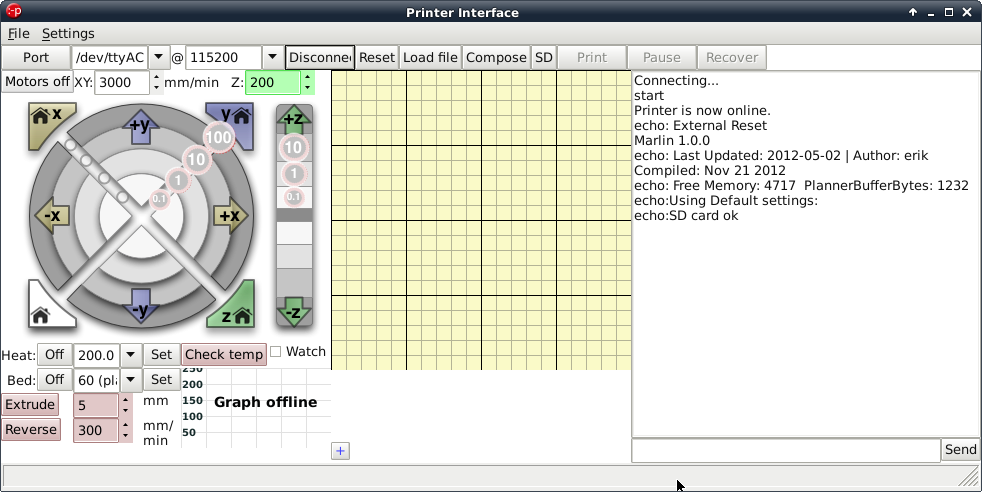
\includegraphics[keepaspectratio=true,angle=0,height=0.4\textheight,width=1.0\textwidth]{printrun.png}
%\caption{Printrun application for 3D printer control}
%\label{fig:Printrun}
%\end{figure}
%The host controls include: setting the extruder and print surface temperatures, manual control of each axis, and manual extrusion. The host is also where you can push print files (\texttt{.gcode}) to the 3D printer or load print files from the SD card for printing out model designs.

%\subsection{Installing Printrun}
%Printrun contains several different applications that can be used to control the Mini 3D printer. It can be installed on Windows, Mac OSX and Linux based computers. Pronterface is the graphical user interface for Printrun. \texttt{Pronsole} allows printing from the command line, and can be used for scripting and some automation. \texttt{Plater} allows you to arrange and combine several STL files into one. More information on the other programs within the Printrun package can be found at \texttt{https://github.com/kliment/Printrun}. Printrun can be downloaded from \texttt{LulzBot.com/support/downloads}. Download the version for your operating system and extract. You will need an archive manager to extract the files. If you do not have one installed we recommend using 7-zip, which can be downloaded for free at \texttt{www.7-zip.org}.

%\begin{itemize}
%\subsection{Windows Instructions}
%\index{windows}
%\item Once downloaded, extract the \texttt{dist} folder to a location of your choice. You can rename the \texttt{dist} folder if you like. Double click \texttt{pronterface.exe} to run Pronterface.


%\subsection{Mac OSX Instructions}
%\item Once downloaded, extract the \texttt{dist} folder to a location of your choice. Once extracted, double click the \texttt{pronterface-mac.app} file to install.

%\subsection{Linux Instructions}
%\begin{itemize}
%\subsubsection{Debian|Ubuntu}
%\subsubsection{Recommended Installation}
%\item We recommend using the stand-alone Printrun option found at \texttt{https://www.LulzBot.com/?=support/downloads}. Once downloaded and extracted, navigate to the extracted directory. Install the dependencies by issuing the following command in a terminal: \texttt{sudo apt-get install python-serial python-wxgtk2.8 python-pyglet}. Once the dependencies have been installed, run Pronterface by using the following command in a terminal: \texttt{python pronterface.py}.

%\subsubsection{Installing from source}
%\item Using Git, in a terminal issue the following command: \texttt{git clone https://github.com/kliment/printrun.git}
%\item Once downloaded, change to the Printrun directory. You will need to ensure that the following dependencies are met. They are listed in the README.md file. You can use this command to install the dependencies: 
%\texttt{sudo apt-get install python-serial python-wxgtk2.8 python-pyglet python-tornado python-setuptools python-libxml2 python-gobject python-pip avahi-daemon libavahi-compat-libdnssd1}
%followed by:
%\texttt{pip install -r requirements.txt}
%To install in a terminal issue the following command:
%\texttt{sudo python setup.py install}.
%Run Printrun by issuing the following command:
%\texttt{python pronterface.py}

%\subsubsection{Fedora}
%\item Use this command to install Printrun from the official sources: \texttt{sudo yum install printrun}

%\subsubsection{Archlinux}
%\item Use this command to install Printun from AUR: \texttt{yaourt rintrun}

%\end{itemize}

%\index{Printrun}
%\section{Using Printrun}

%\begin{figure}[hbt]
%\begin{figure}[H]
%\centering
%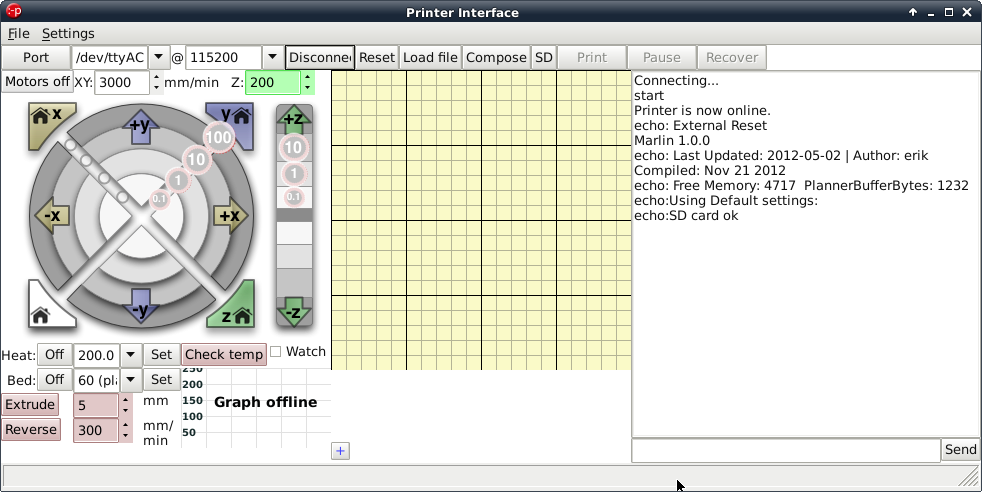
\includegraphics[keepaspectratio=true,angle=0,height=0.4\textheight,width=1.0\textwidth]{printrun.png}
%\caption{Printrun}
%\label{fig:Printrun}
%\end{figure}

%Printrun is used to control the printer from a computer. It is divided into 4 main parts: The buttons over the top are used to connect to the printer, load files and start \& stop prints.

%The movement controls are on the left hand side, with the G-code preview window in the center and the Log %window and Terminal command entry box on the right hand side (Figure \ref{fig:Printrun}, page \pageref{fig:Printrun}).

%\subsection{Connecting to the Mini 3D Printer}
%\index{connecting}
%\index{Printrun}
%\index{USB cable}
%\index{port}
%\index{baud rate}
%\glossary{Baud Rate}{Refers to the speed at which the host controller communicates with the 3d Printer electronics.}
%To start up the printer, first you will need to connect to the printer with Printrun. Make sure you have connected the USB cable from your PC to the printer before launching Printrun. If not, close Printrun, connect the USB cable, and relaunch Printrun. To connect to the printer, select the correct port by using the drop down arrow and selecting the active port, generally \texttt{/dev/ttyACM0}). On other operating systems the port may be named such as \texttt{COM1} or \texttt{tty.usbserial-USB-ID}. The \texttt{Port} button will refresh the Port listing. Once selected choose the default \texttt{115200} buad rate and press \texttt{Connect}. Pronterface will open a connection to the printer and display firmware information in the Log window. 

%In the text output window you will see multiple return lines. If you see \texttt{Printer is now online} you have successfully connected to the printer. The printer control buttons on the left will also darken and become click-able after connecting. If nothing is displayed in the Log window verify you have the correct port and connection speed selected. When you need to disconnect the printer simply press the \texttt{Disconnect} button.

%\begin{figure}[hbt]
%\begin{figure}[H]
%\centering
%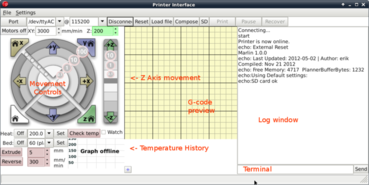
\includegraphics[keepaspectratio=true,angle=0,height=0.4\textheight,width=1.0\textwidth]{printrun-labels.png}
%\caption{Printrun Functions}
%\label{fig:Printrun-labels}
%\end{figure}

%\subsection{Movement} 
%\begin{figure}[hbt]
%\begin{figure}[H]
%\centering
%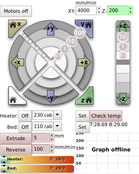
\includegraphics[keepaspectratio=true,angle=0,height=0.4\textheight,width=1.0\textwidth]{printrun_controls.png}
%\caption{Movement Controls}
%\label{fig:Printrun_controls}
%\end{figure}

%\subsubsection{Motors off}
%The Mini 3D printer can be moved on all three axes independently. If you would like to do so by hand, use the \texttt{Motors off} button to unlock all the stepper motors. Once unlocked they can be moved by hand. Keep in mind that there is no positional feedback, so if you move an axis you will need to re-home in order to re-establish the hot end's position. 

%\subsubsection{mm/min XY:/ Z:}
%These settings control the manual jog speeds when driven with Pronterface. Use caution when changing these figures. Moving the axes too fast can cause the printer to miss steps. If that occurs with the Z axis, it can potentially cause the Z axis to become out of square.

%\subsubsection{Homing}
%\index{end stops}
%Caution: when homing, the axis will continue to move in the negative direction until the end stop switch is activated. If the printer is ever transported make sure the end stop switches are clear before resuming printing. If an axis has missed an end stop and is continuing to try to move in the negative direction, immediately turn the power switch to the off position. 

%Each axes can be homed either individually or together. Press the \texttt{Home X} button to move the X axis to the left until it activates the end stop. Once the X axis end stop is activated, the X axis carriage will 'bounce'- it will move over and move back to the home position more slowly. Press the \texttt{Home Y} button to home the Y axis. The Y axis platform will move away from you towards the rear of the printer. The Z home button functions the same, but the Z trigger cannot be adjusted manually on the printer and uses the automatic bed-compensating routine at the beginning of each print.

%\subsubsection{X/Y/Z Axes Movement Controls}
%Prior to moving the X, Y, or Z axis, make sure that you home each axis. The X, Y and Z axes can be moved utilizing the circular movement controls. Each axis can be moved in either fine moves or large moves, ranging from 0.1mm to 100mm.  For example, to move the \texttt{Y Axis} towards you, move your mouse to the \texttt{+y} section until both the \texttt{+y} and the \texttt{100} are highlighted then select that ring section. To move the \texttt{Y axis} away from you, move your mouse to the \texttt{-y} section until both the \texttt{-y} and the \texttt{100} are highlighted then select that ring section. The X axis can be moved in a similar fashion.

%The Z axis movement control operates similarly, but the movement scale is different. The Z axis will move in 0.1mm, 1mm and 10mm increments. The top half of the movement bar will move the Z axis up, by the selected units, while the lower half will move the Z axis down, by the selected units. 




\begin{comment}
\section{Slic3r}
\index{gcode}
\index{STL}
\glossary{STL}{stereolithography file, also known as standard tessellation language; STL file is the common 3D model file format.}
\index{CAD}
\index{resolution}
\index{Slic3r}
Website:  \texttt{http://www.slic3r.org}

The Slic3r software is the first tool in the chain of 3D printing software
(Figure \ref{fig:slic3r}, page \pageref{fig:slic3r}).
\begin{figure}[hbt]
\centering
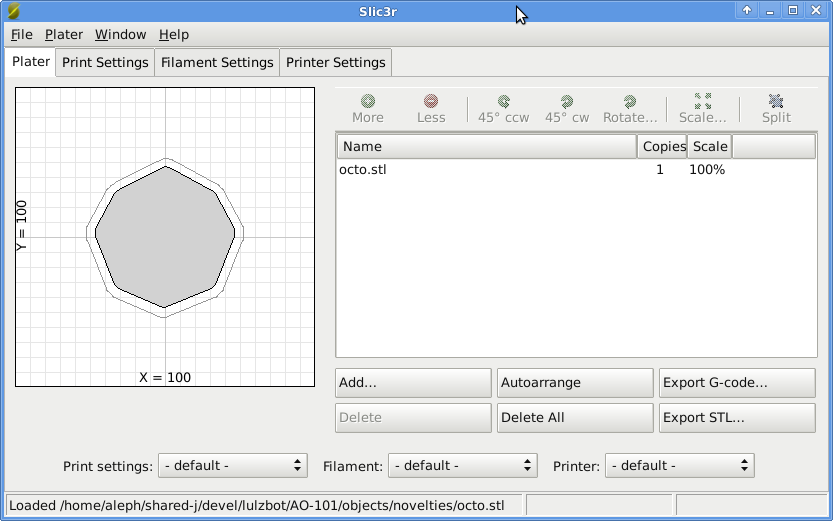
\includegraphics[keepaspectratio=true,angle=0,height=0.4\textheight,width=1.0\textwidth]{slic3r.png}
\caption{Slic3r application, STL to .gcode generator}
\label{fig:slic3r}
\end{figure}

Slic3r uses commonly used \texttt{.STL} files to create \texttt{.gcode} files. Gcode files contain instructions for the 3D printer on where, when, and how quickly to make movements. However, .gcode programming is not very suitable for CAD and 3D design. This is where Slic3r and the \texttt{.STL} file comes into use. The \texttt{.STL} file is a 3D model file that can be exported by all common CAD and 3D modeling software. The Slic3r software then slices the \texttt{.STL} 3D model into layers and print paths to create a 3D-printable \texttt{.gcode} file.

To launch Slic3r navigate to the \texttt{Slic3r} directory and launch the \texttt{slic3r.pl} file. On GNU/Linux operating systems you may need to set the \texttt{slic3r.pl} file as executable. It may be called \texttt{slic3r.exe} on other operating systems.

\index{download}
Slic3r includes very simple settings that allow you to easily refine prints. You can create multiple configurations for changing printer setups including nozzle sizes and desired print resolution. For ease of use we have pre-defined Slic3r configurations. They are available in the Support/Downloads section at \texttt{www.LulzBot.com}. Download the configurations to your \texttt{Slic3r} directory.

\index{configuration}
\subsection{Loading Configurations}
To load configurations, press the \texttt{Load Config...} button. In the file browser that opens, locate the downloaded configuration files. Select the configuration file that matches the nozzle size currently installed on the printer (0.5-mm nozzle is installed by default). Press \texttt{Open} and the pre-defined configuration will load into Slic3r. You can also save custom configurations for yourself by pressing the \texttt{Export Config...} button. A file browser will open that allows you to define a name and save your custom configuration. 

\index{STL}
\index{plater}
\subsection{Loading .STL files}
To load an \texttt{.STL} 3D model file into Slic3r, activate the Plater tab and click the \texttt{Add...} button. In the file browser navigate to the \texttt{.STL} you wish to load and click \texttt{Open}. The silhouette of the model will appear in the Plater diagram. To print more than one copy of the model at a time, select the model name from the list and click the \texttt{More} button. With each press of the \texttt{More} button, an additional copy of the model will be added to Plater. To remove a copy of the model, select the model name again and click \texttt{Less}. To completely remove the model from Plater, select the model name and click \texttt{Delete}.

\index{gcode}
\subsection{Export .gcode files}
Once you have finished setting your part(s) in Plater you can generate the .gcode by clicking \texttt{Export G-Code...}. In the file browser, navigate to where you would like to save the \texttt{.gcode} file and list a name to save the file as. Click \texttt{Save} and Slic3r will begin generating the \texttt{.gcode} file. When Slicer is finished you will receive a prompt. If you have created a plate with multiple model designs, you can also use the \texttt{Export STL...} function to save an \texttt{.STL} file to quickly reproduce the same plate of models.


\section{Printrun}
%%% XXX shouldn't have to do it this way.
%%% HOWTO get page number from section? Ala  sec:Printrun
\label{Printrun}
\index{extruder}
\index{extrusion}
\index{temperature}
\index{gcode}
\index{SD card}
\index{Printrun}
Website: \texttt{http://www.github.com/kliment/Printrun}

The host software, Printrun, can be used to start up and control your 3D printer 
(Figure \ref{fig:Printrun}, page \pageref{fig:Printrun}).
\begin{figure}[hbt]
\centering
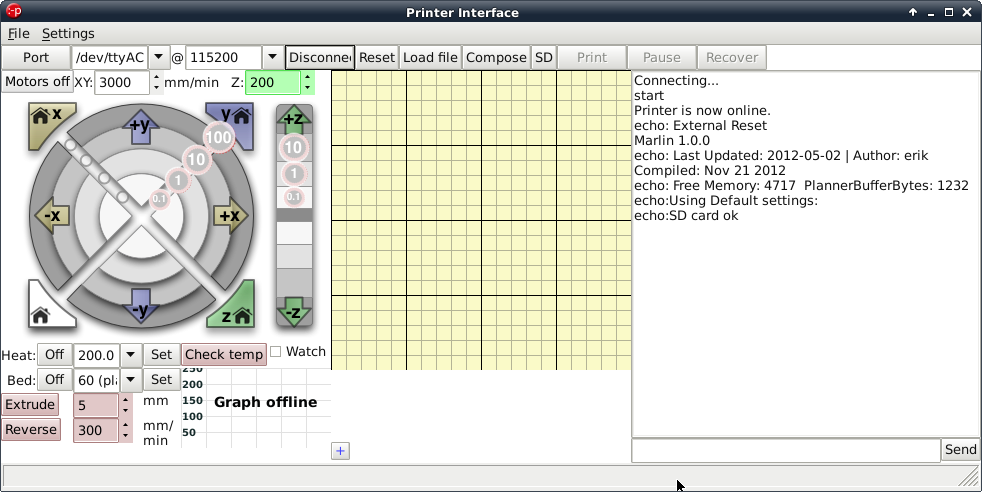
\includegraphics[keepaspectratio=true,angle=0,height=0.4\textheight,width=1.0\textwidth]{printrun.png}
\caption{Printrun application for 3D printer control}
\label{fig:Printrun}
\end{figure}
The host controls include: setting the extruder and print surface temperatures, manual control of each axis, and manual extrusion. The host is also where you will push print files (\texttt{.gcode}) to the 3D printer or load print files from the SD card for printing model designs.

\index{pronterface}
\index{GNU/Linux}
To launch Printrun, navigate to the \texttt{Printrun} directory and launch the \texttt{pronterface.py} file. On GNU/Linux operating systems you may need to set the \texttt{pronterface.py} file as executable. Depending on your environment you may need to launch the program by using the full command: \texttt{python pronterface.py}. On other operating systems the file may be called \texttt{pronterface.exe}.

\subsection{Connecting the Printer}
\index{connecting}
\index{Printrun}
\index{USB cable}
\index{port}
\index{baud rate}
\glossary{Baud Rate}{Refers to the speed at which the host controller communicates with the 3d Printer electronics.}
To start up the printer, first you will need to connect to the printer with Printrun. Before launching Printrun, make sure you have connected the USB cable from your PC to the printer. If not, close Printrun, connect the USB cable, and relaunch Printrun. In the top left \texttt{Port}, pull-down menu select the correct port for the printer (generally \texttt{/dev/ttyACM0}). On other operating systems the port may be named \texttt{COM1} or \texttt{tty.usbserial-USB-ID}. If you have only one printer connected, there will only be one port available to select. Make sure the port baud rate is set to \texttt{115200} in the pull-down menu to the right of the port selection. You can refresh the USB ports, by clicking the \texttt{Port} button.

Now, to connect to the printer, click the \texttt{Connect} button. In the text output window you will see multiple return lines. If you see \texttt{Printer is now online} you have successfully connected to the printer. The printer control buttons on the left will also darken and become click-able after connecting. When you need to disconnect the printer simply press the \texttt{Disconnect} button.

\subsection{Printer Controls}
\index{Printrun}
\index{hot end}
All of the printer controls can be found on the left side of the Printrun interface
(Figure  \ref{fig:Printrun_controls}, page \pageref{fig:Printrun_controls}).
\begin{figure}[hbt]
\centering
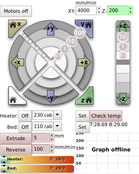
\includegraphics[keepaspectratio=true,angle=0,height=0.4\textheight,width=1.0\textwidth]{printrun_controls.png}
\caption{Printrun controls}
\label{fig:Printrun_controls}
\end{figure}
To set the hot end and print surface temperature, first click the \texttt{Monitor Printer} check box on. This will enable the printer temperature bars and graph. The hot end and print surface controls are labeled \texttt{Heater} and \texttt{Bed}. Select the temperature setting by using the pull-down menu for pre-defined temperature settings. You can also set custom temperature settings by typing into the temperature box.

\index{temperature}
To turn on the hot end and/or printer surface, click the respective \texttt{Set} button. The \texttt{Set} button will highlight orange when the temperature is set to "On" for that component. When the hot end or print surface is set to "On" you will see the temperature bar and graph display the set temperature and the current temperature. When both components have reached the correct temperature, the printer is ready for printing. Clicking the \texttt{Off} button will turn off that component and highlight the \texttt{Off} button blue.

\index{extrude}
\index{hot end}
Below the temperature controls are the manual extrusion controls. There you can manually extrude plastic through the hot end and retract the plastic filament from the hot end. The \texttt{Extrude} button will feed the amount of plastic, set to the right in millimeters, into the hot end. The rate at which the plastic is fed is set below the extrusion length (mm/min). The \texttt{Reverse} button will perform the opposite of \texttt{Extrude}, pulling the plastic filament back out of the hot end.

\index{manual controls}
\index{axes}
\index{X axis}
\index{Y axis}
\index{Z axis}
The large pattern of buttons above the temperature controls are the axes manual controls. These functions allow you to manually move each of the three axes of the printer. The circular pattern of four quadrants controls the X and Y axes. The top and bottom quadrants move the Y axis; the top in the positive direction (forward) and the bottom in the negative direction (backward). The left and right quadrants move the X axis; the left in the negative direction (left) and the right in the positive direction (right).

Each quadrant is split into four sections that control the length of movement by 0.1mm, 1mm, 10mm, or 100mm. The innermost section moves the axis 0.1-mm, with each section outwards becoming a larger movement, with the outside section moving the axis 100-mm.

The linear control bar to the right controls the Z axis. The Z axis is also separated into multiple movement lengths: 0.1mm, 1mm, and 10mm. The upper three buttons move the Z axis up and away from the printer surface; the three lower buttons move the Z axis closer to the print surface.

\index{home}
The four triangular buttons around the circular pattern are the axes home buttons. Each home button will move that axis in the negative direction until the end stop is activated. There is a home button for the X, Y, and Z axes. There is also a white "Home ALL" button that homes all of the axes at once.
\end{comment}


\begin{comment}
\subsection{Loading print files}
\index{load files}
\index{gcode}
\index{Printrun}

To load a \texttt{.gcode} file into Printrun click the \texttt{Load file} button. Navigate to the \texttt{.gcode} file in the file browser and click \texttt{Open}. You will now see a 2D image of the first layer of your model design in the .gcode viewer
(Figure \ref{fig:Printrun_viewer}, page \pageref{fig:Printrun_viewer}).
\begin{figure}[hbt]
\centering
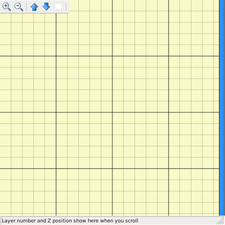
\includegraphics[keepaspectratio=true,angle=0,height=0.4\textheight,width=1.0\textwidth]{printrun_viewer.png}
\caption{Printrun viewer}
\label{fig:Printrun_viewer}
\end{figure}
Click the .gcode viewer window to see a more detailed version of the sliced model. In the pop-up .gcode viewer you can zoom in using the mouse scroll wheel and flip through layers with the up and down arrow keys. To pan within the window, left-click and drag to move around the work plane. The lines shown in the .gcode viewer represent the path the extrusion nozzle will follow to print the model.

For more information on using Printrun, see the Printrun page in the Support/Downloads section at \texttt{https://www.lulzbot.com/?q=support}. Instructions for running a print can be found in the Starting the First Print section in this manual.
\end{comment}

\section{CAD and 3D Modeling Software}
\index{CAD}
\index{software}
\index{STL}

LulzBot is not distributing a CAD or 3D modeling software package. However, multiple free/libre software packages are available. Other common non-free CAD and 3D modeling software are also capable of exporting the required \texttt{.STL} files.

On some CAD and 3D modeling software you will need to select millimeters as the output unit. If possible it is best to build your 3D design in metric units rather than imperial units. Slic3r requires .STL files sized in millimeters. If an .STL with inches as units is loaded into the Slic3r, the model will be scaled much smaller than expected. You can scale the model by 2540\% to compensate. The software listed below outputs millimeters as the unit by default.

\subsection{FreeCAD}
\index{FreeCAD}
\index{GNU/Linux}
\index{Windows}
\index{Apple OS X}
Website: \texttt{http://free-cad.sourceforge.net}

Although still in development, FreeCAD is a great free/libre CAD application. Containing a full GUI for building CAD models, FreeCAD is capable of creating simple to complex designs. STL files can also easily be exported for use with 3D printing. FreeCAD is available for GNU/Linux, Windows, and Mac. The latest development version is recommended.

\subsection{OpenSCAD}
\index{OpenSCAD}
\index{GNU/Linux}
\index{Windows}
\index{Apple OS X}
Website: \texttt{http://openscad.org}

OpenSCAD is another free/libre CAD software; however, different than FreeCAD, it is script based. Rather than using a GUI to generate CAD designs, OpenSCAD CAD designs are created using script based renderings. Users with programming experience would find this very useful. Also, OpenSCAD uses a simple script language that is easy for users with little or no programming experience to learn.

\subsection{Blender}
\index{Blender}
\index{GNU/Linux}
\index{Windows}
\index{Apple OS X}
Website: \texttt{http://blender.org}

The most widely used free/libre 3D modeling software, Blender is well documented with tutorials available on the Blender.org website as well as found online.

\subsection{Shapesmith}
\index{Shapesmith}
Website: \texttt{http://shapesmith.net}

Shapesmith is a web-based 3D modeling software. This means there is no required software to get started designing models. Shapesmith is also a great choice for anyone starting out in CAD/ 3D modeling.

\section{Alternative Printer Host Software}
\index{Host}
\index{software}
\index{STL}

\subsection{OctoPrint}
\index{OctoPrint}
\index{GNU/Linux}
\index{Windows}
\index{Apple OS X}
Website: \texttt{http://octoprint.org/}

Octoprint is a printer host that uses a web-based interface to access and control the 3D printer. Added web-cam functionality allows for time-lapse videos and a live stream. Octoprint will run on Windows, Apple and Linux based computers and can even run well on a Beagle Bone Black or a RaspberryPi (inexpensive business-card sized computers). 

\subsection{BotQueue}
\index{BotQueue}
\index{GNU/Linux}
\index{Apple OS X}
Website: \texttt{https://www.botqueue.com/}

Botqueue works well for those users wanting to have a web-based multiple 3D printer operation running off a queuing system.


\subsection{MatterControl}
\index{MatterControl}
%\index{GNU/Linux}
\index{Windows}
\index{Apple OS X}
Website: \texttt{http://www.mattercontrol.com/}

MatterControl is another printer host that currently runs on Windows and Apple computers. It features 2D and 3D model viewing, a print queue and print file organization and searching.

